\documentclass[a4paper,11pt]{article}
\usepackage{graphicx}
\usepackage{float}
\usepackage{subfig}
\usepackage{subcaption}
\usepackage{geometry}
\usepackage{amsmath,amssymb}
\usepackage{amsthm}
\usepackage{bbold}
\usepackage{mathtools}
\usepackage{braket}
\usepackage{booktabs}
\usepackage[table,xcdraw]{xcolor}
\usepackage[utf8]{inputenc}
\usepackage{cite}
\usepackage[english]{babel}
\usepackage{lipsum}
\usepackage{setspace}
\usepackage{minted}
\usepackage{xcolor}
\newcommand{\R}{\mathbb{R}}
\usepackage{hyperref}
\hypersetup{colorlinks=true,linkcolor=blue}
\geometry{a4paper, top=2.5cm, bottom=2.5cm, left=2cm, right=2cm}

\begin{document}
	\author{Catalano Giuseppe, Cerrato Nunzia}
	\title{Numerical Linear Algebra Homework Project 5:\\Constrained Optimization}
	\date{}
	\maketitle

\section*{Exercise 1}
We want to minimize the function
\begin{equation}
	f_a(\textbf{x}) = (x_{1}-4)^2 + x_{2}^{2}
	\label{eq:func_a}
\end{equation}
subject to the constraints
\begin{equation}
	x_{1} + x_{2} \le 2, \quad x_{1} \ge 0, \quad x_{2} \ge 0,
	\label{eq:constr_a}
\end{equation}
which identify the set $\mathcal{C}_a = \{ \textbf{x} \in \R^2 : x_{1} + x_{2} \le 2, \ x_{1} \ge 0, \ x_{2} \ge 0 \}$. In other words, we want to find 
\begin{equation}
	f_a(\textbf{x}^*) = \min_{\textbf{x} \in \mathcal{C}_a} f_a(\textbf{x}).
\end{equation}
\noindent Since the function $f_a(\textbf{x})$, reported in Eq.~\eqref{eq:func_a}, is convex and continuous and the constraint set $\mathcal{C}_a$ is convex, there exists a unique minimum. In particular, it can be seen that, since there are no mixed terms in $x_1 x_2$ in the expression of the function, its minimum can be found by minimizing $(x_{1}-4)^2$ and $x_{2}^{2}$ separately. $x_{2}^{2}$ is minimized when $x_{2} = 0$, which is compatible with the constraint set, and $(x_{1}-4)^2$ is minimized when $ x_{1} = 4$, which is incompatible with the constraint set. Since it has to be $x_{1} + x_{2} \le 2$, the optimal choice of $x_1$ is $x_1 = 2$. Therefore we have:
\begin{equation}
	\textbf{x}^* = (2,0),\qquad  f_a(\textbf{x}^*) = 4.
\end{equation}
\noindent We would like to find the minimum value both analytically, by solving the KKT system, and numerically, by using the interior point method.\\

\noindent The Lagrangian of the problem is the following:
\begin{equation}
	\mathcal{L}_a(\textbf{x},\boldsymbol{\lambda}) = f_a(\textbf{x}) - \boldsymbol{\lambda}^T \textbf{c}_a(\textbf{x}), \quad \text{with } \textbf{c}_a(\textbf{x}) = \begin{bmatrix}
		2 - x_1 - x_2\\
		x_1\\
		x_2
	\end{bmatrix},
\end{equation}
where the constraints of the problem are satisfied when $c_i(\textbf{x})\ge 0,\ i = 1,2,3$. From this definition, it is possible to write the KKT conditions, namely:
 
\begin{equation}
	\begin{cases}
	\begin{array}{c l}
	\text{stationarity} & (2(x_{1}-4) + \lambda_{1} -\lambda_{2}, 2x_{2}+\lambda_{1}-\lambda_{3}) = (0,0) \\
	\text{primal feasibility} &(2 - x_{1} -x_{2}, x_{1}, x_{2}) \ge (0,0,0) \\
	\text{dual feasibility} & (\lambda_{1}, \lambda_{2}, \lambda_{3}) \ge (0,0,0) \\
	\text{complementarity} &(\lambda_{1}(2-x_{1}-x_{2}), \lambda_{2}x_{1}, \lambda_{3}x_{2}) = (0,0,0)
	\end{array}
	\end{cases}
	\label{eq:KKT system f_a}
\end{equation}
where the inequalities must be intended element-wise.\\

\noindent The complementarity conditions can be satisfied in eight different cases, depending on the fact that each constraint can be active or not. We recall that a constraint $c_{i}(\textbf{x})$ is active if and only if $c_{i}(\textbf{x}^*)=0$.
In the following, we identify each case with an array of $m$ entries, where $m$ is the number of constraints, and we assign to the i-th entry the label $A$ or $N$ depending on whether the i-th constraint is active or not. Associated to each case we report the possible solutions of the constrained minimization problem which are compatible with the corresponding complementarity condition.

\begin{table}[H]
	\centering
	\begin{tabular}{|c|c|c|}
		\hline
		& $A/N$ constraints & Possible solutions $\textbf{x}^*$ \\
		\hline
		1 & $(A, N, N)$ & $\textbf{x}^* = (x_{1}^*,-x_{1}^*+2)$, with $x_{1}^*\in (0,2)$\\
		2 & $(A, A, A)$ & $\nexists \ \textbf{x}^* \in \mathbb{R}^{2}$\\
		3 & $(N, N, N)$ & $\textbf{x}^* \in \mathring{\mathcal{C}}_{a}$\\
		4 & $(N, A, A)$ & $\textbf{x}^* = (0,0)$\\
		5 & $(A, A, N)$ & $\textbf{x}^* = (0,2)$\\
		6 & $(A, N, A)$ & $\textbf{x}^* = (2,0)$\\
		7 & $(N, A, N)$ & $\textbf{x}^* = (0,x_{2}^*)$, with $x_{2}^* \in (0,2)$\\
		8 & $(N, N, A)$ & $\textbf{x}^* = (x_{1}^*,0)$ with $x_{1}^* \in (0,2)$\\
		\hline
	\end{tabular}
	\caption{Table of the cases satisfying the complementarity condition. The i-th row of the table contains the array of the active/non-active states of the constraints (second column) and the possible solutions $\textbf{x}^*$ of the constrained minimization problem which are compatible with that case (third column).}
	\label{tab:complementarity conditions f_a}
\end{table}
\noindent We want to find the solutions to the KKT system \eqref{eq:KKT system f_a} by investigating if the conditions on Lagrange multipliers imposed by the constraint states and the range of possible solutions $\textbf{x}^*$ reported in Tab.~\ref*{tab:complementarity conditions f_a} are compatible with the other equations of the system.
%More specifically, we set to zero the Lagrange multipliers associated with the non-active constraints and we replace all the values in the first two equations.
The results that we find are reported below.
\begin{enumerate}
	\item From the case $(A,N,N)$ we have $ \lambda_{2}^*=\lambda_{3}^*=0$. This leads to $\lambda_{1}^*=2$ and $\textbf{x}^*=(3,-1)$, which is not compatible with the constraint set.
	\item For the case $(A,A,A)$ it can be seen from the second row of the Table \ref{tab:complementarity conditions f_a} that $\nexists \ \textbf{x}^* \in \mathbb{R}^{2}$ which represents a solution to the constrained minimization problem.
	\item From the case $(N,N,N)$ we have $\lambda_{1}^*= \lambda_{2}^*= \lambda_{3}^*=0$. In this case, one finds $\textbf{x}^* = (4,0)$, which is outside the feasible set.
	\item From the case $(N,A,A)$ we have $\lambda_{1}^*=0$. From the complementarity condition we already have $\textbf{x}^*=(0,0)$. From the stationarity condition, we find $\lambda_{3}^*=0$, and $\lambda_{2}^*=-8$, which is not allowed.
	\item From the case $(A,A,N)$ we have $\lambda_{3}^*=0$. From the complementarity condition we already have $\textbf{x}^*=(0,2)$. By inserting this value in the first equation of the KKT system, we find $\lambda_{1}^*=-4$, $ \lambda_{2}^*=-12$, which are both not allowed values.
	\item From the case $(A,N,A)$ we have $\lambda_{2}^*=0$. In this case, one has $\textbf{x}^*=(2,0)$ from the complementarity condition and $\lambda_{1}^*=4$, $\lambda_{3}^*=4$, which are both acceptable solutions. Note that this is the solution that we have already found heuristically.
	\item From the case $(N, A, N)$ we have $\lambda_{1}^*=0,\ \lambda_{3}^*=0$. In this case, we find $\lambda_{2}^*=-8$, which is not an acceptable solution.
	\item From the case $(N, N, A)$ we have $\lambda_{1}^*=0,\ \lambda_{2}^*=0$. In this case, we find $\lambda_{3}^*=0$ and $\textbf{x}^*=(4,0)$, which is outside the feasible set.
\end{enumerate}

\noindent As emerges from the study of the KKT system, $\boldsymbol{\lambda}^*=(4,0,4)$ and the unique solution to the constrained minimization problem is $\textbf{x}^*=(2,0)$, where $f_{a}(\textbf{x}^*) = 4$.

\section*{Exercise 2}
We want to minimize the function
\begin{equation}
	f_{b}(\textbf{x})=2x_{1} - x_{2}^2,
	\label{eq:func_b}
\end{equation}
under the constraints
\begin{equation}
	x_{1}^2 + x_{2}^2 \le 1, \quad x_{1}\ge0, \quad x_{2}\ge0,
	\label{eq:constr_b}
\end{equation}
which identify the set $\mathcal{C}_{b} = \{\textbf{x}\in \mathbb{R}^2 : x_{1}^2 + x_{2}^2 \le 1, \ x_{1}\ge0,\ x_{2}\ge0 \}$. In other words, we want to find
\begin{equation}
	f_b(\textbf{x}^*) = \min_{\textbf{x} \in \mathcal{C}_b} f_b(\textbf{x}).
	\label{eq:min_prob_func_b}
\end{equation}
In this case, the function $f_b(\textbf{x})$ is concave, therefore, in principle, nothing can be said about its minimum. However, by exploiting the constraints, we can obtain the following chain of inequalities
\begin{equation}
	f_b(\textbf{x}) = 2x_{1}-x_{2}^2\ge-x_{2}^2\ge-1,
\end{equation}
where in the first inequality we use $x_{1}\ge0$, which is saturated when $x_{1}=0$, while in the second one we use that $x_{2}^2 \le 1-x_{1}^2\le1$, which is saturated when $x_{2}=\pm1$. Finally, knowing that $x_{2}$ must be positive, we can conclude that the unique solution of the problem in Eq.~\eqref{eq:min_prob_func_b} is $\textbf{x}^*=(0,1)$ and $f_b(\textbf{x}^*)=-1$.\\

\noindent We would like to obtain now the same minimum point by solving the KKT system analytically and, subsequently, by exploiting the interior point method numerically.

\noindent The Lagrangian associated with the problem is the following:
\begin{equation}
	\mathcal{L}_b(\textbf{x},\boldsymbol{\lambda}) = f_b(\textbf{x}) - \boldsymbol{\lambda}^T \textbf{c}_b(\textbf{x}), \quad \text{with } \textbf{c}_b(\textbf{x}) = \begin{bmatrix}
		1-x_{1}^2 - x_2^2\\
		x_1\\
		x_2
	\end{bmatrix},
\end{equation}
where the constraints of the problem are satisfied when $c_i(\textbf{x})\ge 0,\ i = 1,2,3$. The KKT system is:
\begin{equation}
	\begin{cases}
		\begin{array}{c l}
			\text{stationarity} & (2 + 2\lambda_{1}x_{1} -\lambda_{2}, -2x_{2}+2\lambda_{1}x_{2}-\lambda_{3}) = (0,0) \\
			\text{primal feasibility} &(1 - x_{1}^2 -x_{2}^2, x_{1}, x_{2}) \ge (0,0,0) \\
			\text{dual feasibility} & (\lambda_{1}, \lambda_{2}, \lambda_{3}) \ge (0,0,0) \\
			\text{complementarity} &(\lambda_{1}(1-x_{1}^2-x_{2}^2), \lambda_{2}x_{1}, \lambda_{3}x_{2}) = (0,0,0)
		\end{array}
	\end{cases}
	\label{eq:KKT system f_b}
\end{equation}
where the inequalities must be intended element-wise.\\

\noindent Analogously to the previous case, we study the eight cases that can be derived from the complementarity condition. We report in the following table the possible solutions to the constrained minimization problem which are compatible with the corresponding complementarity condition.
\begin{table}[H]
	\centering
	\begin{tabular}{|c|c|c|}
		\hline
		& $A/N$ constraints & Possible solutions $\textbf{x}^*$ \\
		\hline
		1 & $(A, A, A)$ & $\nexists \ \textbf{x}^* \in \mathbb{R}^{2}$\\
		2 & $(A, A, N)$ & $\textbf{x}^* = (0,1)$\\
		3 & $(A, N, A)$ & $\textbf{x}^* = (1,0)$\\
		4 & $(A, N, N)$ & $x_{2}^* = \sqrt{(1-{x_{1}^*}^2)}$, with $x_{1}^* \in (0,1)$\\
		5 & $(N, A, A)$ & $\textbf{x}^* = (0,0)$\\
		6 & $(N, A, N)$ & $\textbf{x}^* = (0,x_{2}^*)$, with $x_{2}^* \in (0,1)$\\
		7 & $(N, N, A)$ & $\textbf{x}^* = (x_{1}^*,0)$ with $x_{1}^* \in (0,1)$\\
		8 & $(N, N, N)$ & $\textbf{x}^* \in \mathring{\mathcal{C}}_{b}$\\
		\hline
	\end{tabular}
	\caption{Table of the cases satisfying the complementarity condition. The i-th row of the table contains the array of the active/non-active states of the constraints (second column) and the possible solutions $\textbf{x}^*$ of the constrained minimization problem which are compatible with that case (third column).}
	\label{tab:complementarity conditions f_b}
\end{table}

\begin{enumerate}
	\item For the case $(A, A, A)$ it can be seen from the second row of the Table \ref{tab:complementarity conditions f_b} that $\nexists \ \textbf{x}^* \in \mathbb{R}^{2}$ which represents a solution to the constrained minimization problem.
	\item For the case $(A, A, N)$ we have $\lambda_{3}^*=0$. From the complementarity condition we already know that $\textbf{x}^*=(0,1)$. By inserting this value in the first equation of the KKT system, we find $\lambda_{1}^*=1$ and $\lambda_{2}^*=2$, which are allowed values.
	\item For the case $(A, N, A)$ we have $\lambda_{2}^*=0$. In this case, we have already found that $\textbf{x}^*=(1,0)$, which leads to $\lambda_{1}^*=-1$, which is not allowed, and $\lambda_{3}^*=0$.
	\item For the case $(A, N, N)$ we have $\lambda_{2}^*=\lambda_{3}^*=0$. From the first equation of the KKT system, we arrive at the condition $\lambda_{1}^* x_{1}^*=-1$, which cannot be satisfied since both $\lambda_{1}^*$ and $x_{1}^*$ must be positive.
	\item For the case $(N, A, A)$ we have $\lambda_{1}^*=0$. Here we already have $\textbf{x}^*=(0,0)$, which leads to $\lambda_{2}^*=2$ and $\lambda_{3}^*=0$.
	\item For the case $(N, A, N)$ we have $\lambda_{1}^*=\lambda_{3}^*=0$. In this case, we find $\lambda_{2}^*=2$ and $\textbf{x}^*=(0,0)$.
	\item For the case $(N, N, A)$ we have $\lambda_{1}^*=\lambda_{2}^*=0$. By inserting these values in the stationarity condition we arrive at the expression $2=0$, which is absurd, therefore no solutions can be found in this case.
	\item For the case $(N, N, N)$ we have $\lambda_{1}^*=\lambda_{2}^*=\lambda_{3}^*=0$. This case is analogous to the previous one since we arrive at the same expression $2=0$ when considering $\lambda_{1}^*=0$, therefore no solutions can be found.
\end{enumerate}
From the analysis of the KKT conditions, we can conclude that there exist two solutions to the KKT system, namely $\textbf{x}_{1}^*=(0,1)$ with $\boldsymbol{\lambda}_{1}^*=(1,2,0)$ and $\textbf{x}_{2}^*=(0,0)$ with $\boldsymbol{\lambda}_{2}^*=(0,2,0)$. By evaluating the function at these points we have $f_{b}(\textbf{x}_{1}^*)=-1$ and  $f_{b}(\textbf{x}_{2}^*)=0$, therefore we conclude that $\textbf{x}_{1}^*$ is the solution of the constrained minimization problem. However, since there are two solutions to the KKT system, we expect there could be problems when searching numerically the minimum of this function by using the interior point method.

\section*{Exercise 3}
Consider the problem
\begin{equation}
	\min f(\textbf{x}) - \mu \textbf{e}^{T}\log(\textbf{z}) \quad \text{s.t.} \quad \textbf{c}(\textbf{x})- \textbf{z} = \textbf{0},
	\label{eq:pert_min_prob}
\end{equation}
where $f : \R^{n} \rightarrow \R$, is the function one wants to minimize, $\textbf{c} : \R^{n} \rightarrow \R^{m}$ is a vector defining the constraints, which are assumed to be $c_{i}(\textbf{x})\ge0, \ \forall i=1,\dots,m$, $\textbf{z}\, \in \R^{m}$ is called slack variable and, finally, $\textbf{e}^{T}=(1,\dots,1)\in \R^{m}$ and $\mu>0$. Due to the presence of the logarithmic term, for sufficiently small values of the parameter $\mu$ this represents a slightly perturbed version of a constrained minimization problem.\\

\noindent In this case, from the KKT theorem it is possible to find the following necessary conditions:
\begin{align}
	& \textbf{r}_{1} \coloneqq \nabla f(\textbf{x}) - \boldsymbol{\lambda}^{T}\nabla_{\textbf{x}}\textbf{c}(\textbf{x}) = \textbf{0} \\
	& \textbf{r}_{2} \coloneqq \textbf{c}(\textbf{x}) - \textbf{z} = \textbf{0} \\
	& \textbf{r}_{2} \coloneqq \textbf{z} \odot  \boldsymbol{\lambda} - \mu \textbf{e} = \textbf{0}.
\end{align}
In order to solve this system, it is necessary to update the variables $\textbf{x}$, $\boldsymbol{\lambda}$, $\textbf{z}$, which can define a new variable $\textbf{y} = [\textbf{x}, \boldsymbol{\lambda}, \textbf{z}]^{T}$. By denoting with $R(\textbf{x})$ the matrix with rows $\textbf{r}_{1}$, $\textbf{r}_{2}$, $\textbf{r}_{3}$, the updating step is

\begin{equation}
	\textbf{y}_{k+1} = \textbf{y}_{k} - \nabla R(\textbf{y}_{k})^{-1} R(\textbf{y}_{k}),
\end{equation}
where $\nabla R(\textbf{y})$ represents the Jacobian of the system, given by:
\begin{equation}
	\nabla R(\textbf{y}) = J(\textbf{x}, \boldsymbol{\lambda},\textbf{z}) =  
	\begin{pmatrix}
		H(\textbf{x}) + K(\textbf{x}, \boldsymbol{\lambda}) & -\nabla\textbf{c}(\textbf{x})^{T} & \textbf{0}_{n\times m}\\
		\nabla\textbf{c}(\textbf{x}) & \textbf{0}_{m\times m} & -\mathbb{1}_{m}\\
		\textbf{0}_{m\times n} & \text{diag}(\textbf{z}) & \text{diag}(\boldsymbol{\lambda})
	\end{pmatrix},
\end{equation}
where $H(\textbf{x}) = \nabla^{2}f(\textbf{x})$, $K(\textbf{x},\boldsymbol{\lambda})=-\boldsymbol{\lambda}^{T}\nabla^{2}\textbf{c}(\textbf{x})$.\\

\noindent We want to write down the Jacobian associated with the problem \eqref{eq:pert_min_prob} considering as functions and constraints the ones of the two previous exercises.

\subsection*{Function $\boldmath{f_{a}}(\textbf{x})$}
We recall the expression of the function $f_{a}(\textbf{x}) = (x_{1}-4)^2 + x_{2}^{2}$ and that of the constraints, which are written in the form $c_{i}(\textbf{x})\ge0$, and can be recast in the vector
\begin{equation}
	\textbf{c}_{a}(\textbf{x}) = 
	\begin{bmatrix}
		2 -x_{1} - x_2\\
		x_1\\
		x_2
	\end{bmatrix}.
\end{equation}
In order to obtain the Jacobian, we have to compute the gradient and the Hessian of the function and the constraints. We report in the following their expressions.

\begin{align}
	& \nabla f_{a}(\textbf{x}) = [2(x_{1}-4),2x_{2}]^{T} \qquad H_{f_{a}}(\textbf{x}) = \begin{bmatrix}
		2 & 0 \\
		0 & 2
	\end{bmatrix}, \\
	& \nabla \textbf{c}_{a}(\textbf{x}) = \begin{bmatrix}
		-1 & - 1\\
		1 & 0 \\
		0 & 1
	\end{bmatrix} \qquad \qquad \nabla^{2}{\textbf{c}_{a}}(\textbf{x}) =  \left[\textbf{0}_{2\times2},\textbf{0}_{2\times2},\textbf{0}_{2\times2}\right]^{T}.
\end{align}
Therefore, $K_{a}(\textbf{x},\boldsymbol{\lambda})=\textbf{0}_{2\times 2}$ as expected, since all the constraints are linear.
\subsection*{Function $\boldmath{f_{b}}(\textbf{x})$}
As before, we recall the expression of the function $f_{b}(\textbf{x}) = 2x_{1} - x_{2}^{2}$ and that of the constraints, which are written also in this case in the form $c_{i}(\textbf{x})\ge0$, and can be recast in the vector
\begin{equation}
	\textbf{c}_{b}(\textbf{x}) = 
	\begin{bmatrix}
		1 -x_{1}^{2} - x_2^{2}\\
		x_1\\
		x_2
	\end{bmatrix}.
\end{equation}
We report in the following the gradient and the Hessian of the function and the constraints:
\begin{align}
	& \nabla f_{b}(\textbf{x}) = [2, -2x_{2}]^{T} \qquad \qquad \qquad \ \ H_{f_{b}}(\textbf{x}) = \begin{bmatrix}
		0 & 0 \\
		0 & -2
	\end{bmatrix}, \\
	& \nabla \textbf{c}_{b}(\textbf{x}) = \begin{bmatrix}
		-2x_{1} & - 2x_{2}\\
		1 & 0 \\
		0 & 1
	\end{bmatrix} \qquad \qquad \nabla^{2}{\textbf{c}_{b}}(\textbf{x}) =  \left[\nabla^{2}[\textbf{c}_{b}]_{1},\textbf{0}_{2\times2},\textbf{0}_{2\times2}\right]^{T},
\end{align}
where $\nabla^{2}[\textbf{c}_{b}]_{1} = -\mathbb{1}_{2}$ and, therefore, $K_{b}(\textbf{x},\boldsymbol{\lambda})=\lambda_{1}\mathbb{1}_{2}$.

\section*{Exercise 4}
We want to implement the interior point method to solve numerically the constrained minimization problems of Exercise 1 and Exercise 2. We used Python as the programming language and we created a file named \mintinline{Python}{Project_5.py}, which can be found at this \href{https://github.com/nunziacerrato/Numerical_Analysis_Optimization/blob/main/Project_5/Project_5.py}{link} on GitHub, where we defined the function \mintinline{Python}{int_point}. We describe below the main characteristics of this function. \\
%
% and we defined the function \mintinline{Python}{int_point}, which can be found in the file \mintinline{Python}{Project_5.py} at this \href{https://github.com/nunziacerrato/Numerical_Analysis_Optimization/blob/main/Project_5/Project_5.py}{link} on GitHub.\\
%

\noindent We pass explicitly to this function the variable \mintinline{Python}{method}, which allows one to choose which method to implement in order to compute the Newton step and we also give the option to choose whether to consider or not the curvature term in the Jacobian. Moreover, for setting the starting values of $\boldsymbol{\lambda}$ and $\textbf{z}$, the function \mintinline{Python}{int_point} accepts both given arrays and the string \mintinline{Python}{'random'}, in such case these arrays are uniformly randomly generated. To ensure reproducibility, we fix the seed, still giving the possibility of changing it by passing a specific value to the corresponding keyword argument.  Finally, we choose as default values for the parameter $\mu$ of the logarithmic barrier the value $\mu = 10^{-12}$, as tolerance parameter the value $10^{-12}$, and $100$ as the maximum number of iterations allowed. Note that these values can be user-changed as they are keyword arguments of the function. All the other details can be found in the documentation. In the following, we report the code.


\begin{minted}[mathescape, linenos, breaklines]{Python}
def int_point(func, grad_func, hess_func, constr, grad_constr, hess_constr, x0, method='basic', alpha=1., beta=1., gamma=1., mu=1e-12, tol=1e-12, maxit=100, l0='random', z0='random', curv=False, seed=1):
   '''This function implements the interior point method for constrained minimization problems.
   Parameters
   ----------
   func : function
      Function to be minimized.
   grad_func : function
      Gradient of the function. It returns a 1d-array (vector)
   hess_func : function
      Hessian of the function. It returns a 2d-array (matrix)
   constr : function
      Function of the constraints. It returns a 1d-array (vector).
   grad_constr : function
      Gradient of the function of the constraints. It returns a 2d-array (matrix)
   hess_constr : function
      Hessian of the function of the constraints. It returns a 3d-array
   x_0 : ndarray
      Starting point
   method : str
      String to choose the method to perform the Newton step. Possible values are
      - 'basic': to solve the full linear system
      - 'first': to solve the first reduced linear system
      - 'full': to solve the fully reduced linear system
      Default value method='basic'.
   alpha : float
      Starting step-lenght for the parameter x. Default value alpha=1.
   beta : float
      Starting step-lenght for the parameter lambda. Default value beta=1.
   gamma : float
      Starting step-lenght for the parameter z. Default value gamma=1.
   mu : float
      Coefficient of the log barrier term
   tol : float
      Tolerance parameter for the stopping criterion. Default value tol=1e-12
   maxit : int
      Maximum number of iterations. Default value maxit=100
   l0 : str or ndarray
      Starting value of the Lagrange multipliers. Deafult value l0='random', to generate uniformly distributed random values in the interval [1e-16,10).
   z0 : str or ndarray
      Starting value of the slack variable. Deafult value z0='random', to generate uniformly distributed random values in the interval [1e-16,10).
   curv : bool
      Boolean value to choose whether to discard (curv=False) or not (curve=True) the curvature term in the expression of the Jacobian of the system. Default value curv=False.
   seed : int
      Parameter to fix the seed. Default value seed=1

   Results
   -------
   results : dict
      Dictionary of the results given by the function. It contains the following items:
      - 'convergence' : (bool) True if the algorithm converges, False if it doesn't converge
      - 'n_iter' : (int) progressive number of final iteration
      - 'x_min' : (ndarray) computed point at which the minimum of the function is reached
      - 'f_min' : (float) computed minimum value of the function
      - 'x_interm' : (list) list of the intermediate points
      - 'lambda_interm' : (list) list of the intermediate Lagrange multipliers
      - 'z_interm' : (list) list of the intermediate slack variables
   '''

   # Check if the starting point is in the feasible set
   if any(constr(x0) < 0):
      print(f'Starting point x0 = {x0} is not feasible')
      return False

   # Assign initial values to the the variables x_old, lambda_old and z_old
   x_old = x0
   lambda_old, z_old = l0, z0
   m, n = len(constr(x_old)), len(x_old)

   # Fix the seed and initialize lambda_old and z_old by using the uniform random distribution if required 
   np.random.seed(seed=seed)
   if type(l0) == str and l0 == 'random':
      lambda_old = np.random.uniform(low=1e-16, high= 10., size=m)
   if type(z0) == str and z0 == 'random':
      z_old = np.random.uniform(low=1e-16, high= 10., size=m)

   # Compute the vector R
   r1 = grad_func(x_old) - lambda_old @ grad_constr(x_old)
   r2 = constr(x_old) - z_old
   r3 = z_old*lambda_old - mu
   R = np.array([*r1, *r2, *r3])

   # Append the starting values of the variables to the corresponding lists
   x_interm = [x0]
   lambda_interm = [lambda_old]
   z_interm = [z_old]

   # Cycle until the stopping criterion is satisfied or k reaches the maximum number of iterations
   k = 0
   while(np.linalg.norm(R)>tol and k < maxit):
      a0, b0, g0 = alpha, beta, gamma

      # Compute matrices and vectors entering the expression of the linear system
      Z = np.diag(z_old)
      Z_inv = np.linalg.inv(Z)
      grad_c = grad_constr(x_old)
      Lambda = np.diag(lambda_old)
      hess_f = hess_func(x_old)
      K = 0
      if curv == True:
         hess_c = hess_constr(x_old)
         K = - lambda_old @ hess_c

      # Choose the method to perform the Newton step and compute dx, dl, dz
      # Solve the full system
      if method == 'basic':            
         Jacobian = np.block([[ hess_f + K, - grad_c.T, np.zeros((n,m)) ],
                              [ grad_c , np.zeros((m,m)), - np.eye(m)],
                              [ np.zeros((m,n)), Z, Lambda ]])
         p = np.linalg.solve(Jacobian, -R)
         dx = p[:n]
         dl = p[n:n+m]
         dz = p[n+m:]

      # Solve the first reduced system
      if method == 'first':
         Lambda_inv = np.linalg.inv(Lambda)
         matrix = np.block([[hess_f + K, -(grad_c).T],
                            [grad_c, Lambda_inv @ Z]])
         vector = np.array([*r1, *(r2 + Lambda_inv @ r3)])

         p = np.linalg.solve(matrix,-vector)
         dx = p[:n]
         dl = p[n:]
         dz = - Lambda_inv @ (r3 + Z @ dl)

      # Solve the fully reduced system
      if method == 'full':            
         matrix = hess_f + K + (grad_c).T @ (Z_inv @ Lambda @ grad_c )
         vect = - r1 - (grad_c).T @ Z_inv @ (r3 + Lambda @ r2)

         dx = np.linalg.solve(matrix,vect)
         dl = - Z_inv @ Lambda @ r2 - Z_inv @ r3 -Z_inv @ Lambda @ grad_c @ dx
         dz = - np.linalg.inv(Lambda) @ (r3 + Z @ dl)

      # Update the values of the variables
      x_new = x_old + a0*dx
      lambda_new = lambda_old + b0*dl
      z_new = z_old + g0*dz

      # Check if the updated values satisfy the required conditions and re-update them until necessary
      while any(constr(x_new) < 0 ):
         a0 = a0/2
         x_new = x_old + a0*dx

      while any(lambda_new < 0 ):
         b0 = b0/2
         lambda_new = lambda_old + b0*dl

      while any(z_new <= 0 ):
         g0 = g0/2
         z_new = z_old + g0*dz

      # Append the new values of the variables to the corresponding lists
      x_interm.append(x_new)
      lambda_interm.append(lambda_new)
      z_interm.append(z_new)

      # Compute the new values of R
      r1 = grad_func(x_new) - lambda_new @ grad_constr(x_new)
      r2 = constr(x_new) - z_new
      r3 = z_new*lambda_new - mu
      R = np.array([*r1, *r2, *r3])

      x_old = x_new
      lambda_old = lambda_new
      z_old = z_new
      k = k + 1

      # Check if the convergence is reached
      conv = True
      if k == maxit:
          conv = False

      f_min = func(x_new)

      results = {'convergence' : conv, 'n_iter' : k , 'x_min' : x_new, 'f_min' : f_min, 'x_interm' : x_interm, 'lambda_interm' : lambda_interm, 'z_interm' : z_interm}
      
      return results
\end{minted}

\subsection*{Function $\boldmath{f_{a}}(\textbf{x})$}
First and foremost, after having chosen a representative starting point, i.e.~$\textbf{x}_{0}=(0.5,0.5)$, we run the function \mintinline{Python}{int_point} by using the three different methods to compute the Newton step, namely \mintinline{Python}{'basic'} which solves the complete linear system, \mintinline{Python}{'first'} which solves the first reduced linear system, and \mintinline{Python}{'full'}  which solves the fully reduced linear system  We report in the following the results that we obtain by choosing the components of $\boldsymbol{\lambda}_{0}$ and $\textbf{z}_{0}$ uniformly distributed in the interval $\left[10^{-16},10\right)$. Note that we use the same vectors $\boldsymbol{\lambda}_{0}$ and $\textbf{z}_{0}$ in all the three cases.
\begin{minted}{text}
convergence = True, with 9 steps and method = basic
starting point = (0.5, 0.5)
mu = 1e-12, lambda_0 = (6.2, 1.4, 3.3), z_0 = (2.8, 5.9, 5.5)
min point = (1.99999999999948, 2.5768276401549883e-13)
min value = 4.00000000000208
lambda_fin = (4.0000000000015214, 4.818155423247372e-13, 4.0000000000020375)
z_fin = (2.6239080128549816e-13, 1.99999999999948, 2.576828630208037e-13)

convergence = True, with 9 steps and method = first
starting point = (0.5, 0.5)
mu = 1e-12, lambda_0 = (6.2, 1.4, 3.3), z_0 = (2.8, 5.9, 5.5)
min point = (1.99999999999948, 2.5768276401549883e-13)
min value = 4.00000000000208
lambda_fin = (4.0000000000015214, 4.818148918034337e-13, 4.0000000000020375)
z_fin = (2.623908012854933e-13, 1.9999999999994804, 2.576828630208021e-13)

convergence = True, with 9 steps and method = full
starting point = (0.5, 0.5)
mu = 1e-12, lambda_0 = (6.2, 1.4, 3.3), z_0 = (2.8, 5.9, 5.5)
min point = (1.99999999999948, 2.576828630208037e-13)
min value = 4.00000000000208
lambda_fin = (4.000000000001522, 4.818155423247372e-13, 4.000000000002037)
z_fin = (2.623908012854933e-13, 1.9999999999994802, 2.576828630208037e-13)
\end{minted}

\noindent We can observe that the three methods converge to the solution with the same number of steps, as expected since they solve equivalent linear systems. The difference between them may be in the time they take to arrive at the solution, due to the fact that they solve systems of different dimensionalities. However, in this case, this difference has not been appreciable as the system that we solve is already of small size. Moreover, as expected, the error on the computed quantities is of $\mathcal{O}(\mu)$ and the values of the components of $\textbf{z}_{fin}$, that is the vector of slack variables in correspondence with the final iteration, are compatible, within this error, with the values of the constraints computed at $\textbf{x}^{*}$, namely $\textbf{c}_{a}(\textbf{x}^{*})=(0,2,0)$.\\

\noindent After this first analysis, we have decided to use the method \mintinline{Python}{'basic'} as we expect this to be the most stable one. We analyze different starting points $\textbf{x}_{0}$ as well as different  values of $\boldsymbol{\lambda}_{0}$ and $\textbf{z}_{0}$. 
In order to present the obtained results, we first consider a fixed starting point and a fixed $\mu$ value, while varying $\boldsymbol{\lambda}_{0}$ and $\textbf{z}_{0}$. Then, for a fixed triad of values $\textbf{x}_{0}$, $\boldsymbol{\lambda}_{0}$, and $\textbf{z}_{0}$, we compare the number of iterations towards convergence for two different $\mu$ values. In all the plots we report the intermediate points as they reach the constrained minimum point.
\begin{figure}[H]
	\centering
	\subfloat[\label{fig:panel_a}]{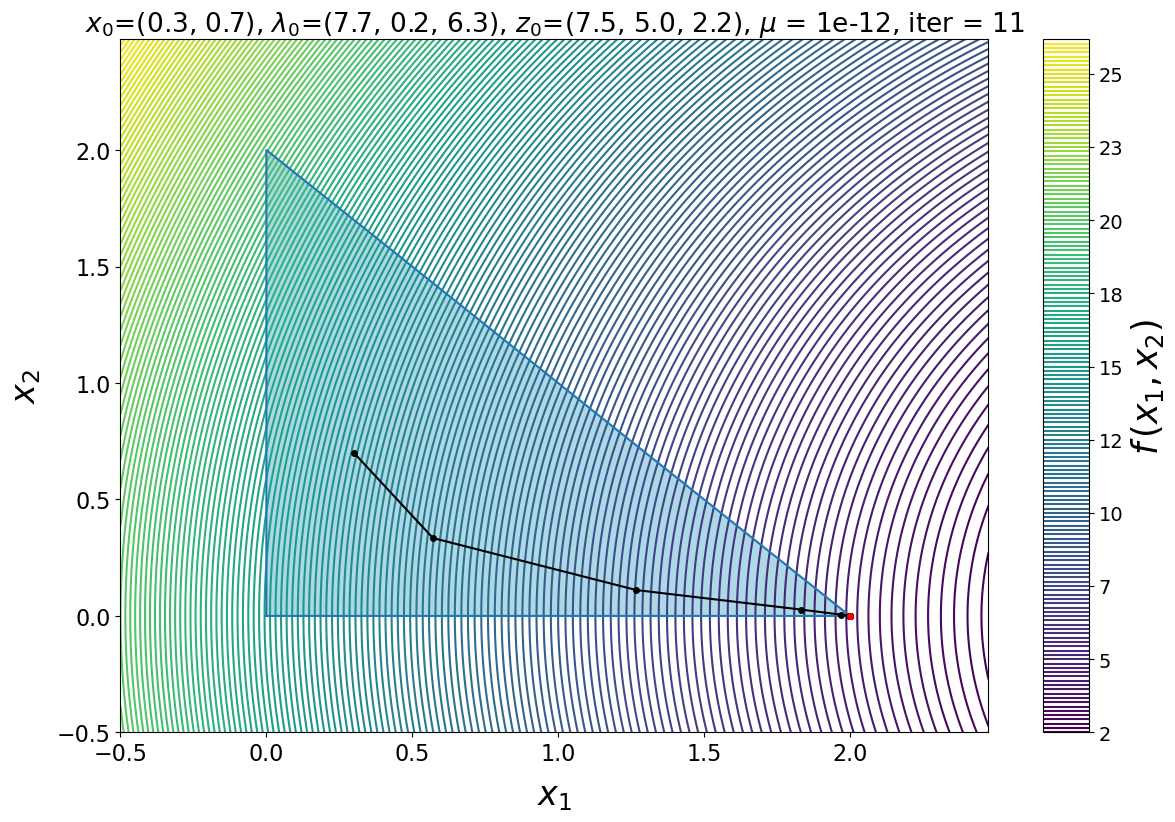
\includegraphics[scale=0.28]{Plot/func_a_method=basic_x0=[0.3 0.7]_mu=1e-12_seed=10.png}}\
	\subfloat[\label{fig:panel_b}]{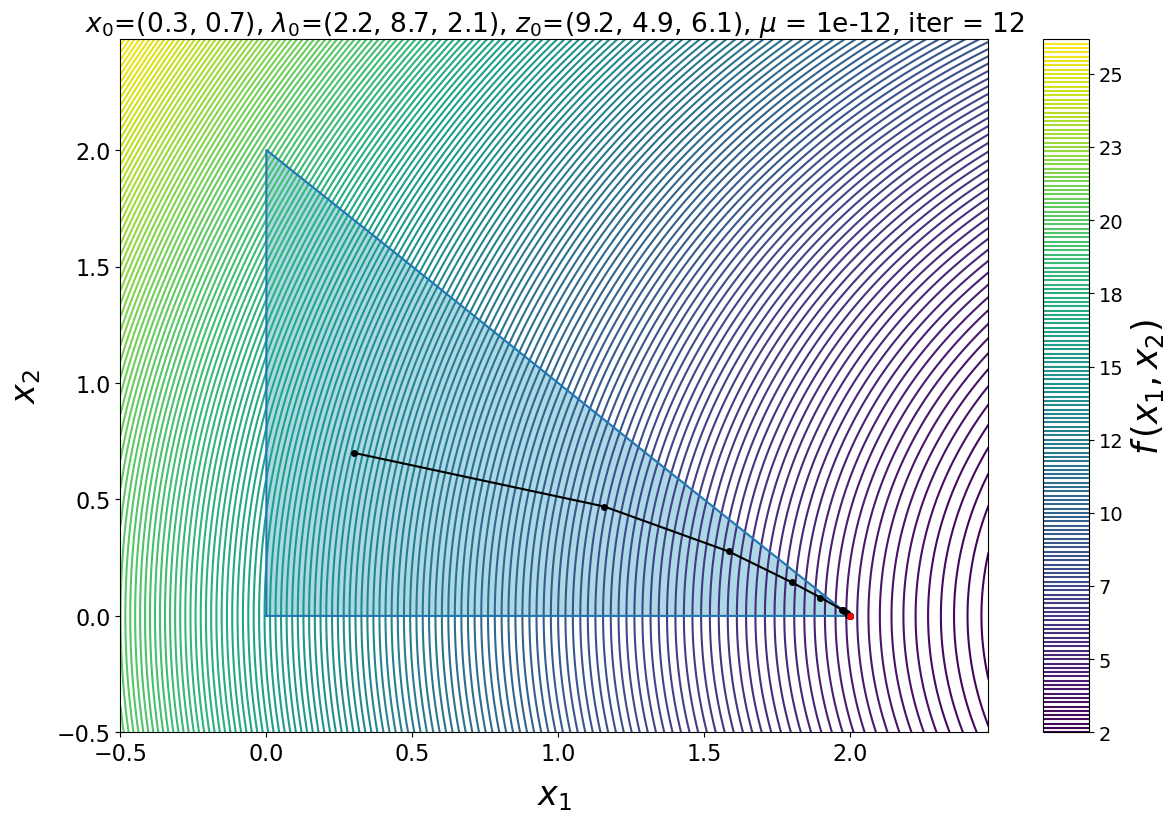
\includegraphics[scale=0.28]{Plot/func_a_method=basic_x0=[0.3 0.7]_mu=1e-12_seed=5.png}}
	\caption{Contour plot of the function $f_{a}(x_{1},x_{2})$ with $\mu=10^{-12}$, for fixed $\textbf{x}_{0}$ and different values of $\boldsymbol{\lambda}_{0}$, and $\textbf{z}_{0}$, reported in the title of the plots. The constrained set is represented by the triangle in blue. In red is the constrained minimum point the interior point algorithm converges to.}
	\label{Fig:func_a}
\end{figure}

\noindent It can be noted that different choices of the initial values of $\boldsymbol{\lambda}$ and $\textbf{z}$ imply, as expected, a different path towards convergence since the descent direction depends on them. On the other hand, we also expect that, for a fixed value of $\boldsymbol{\lambda}$ and $\textbf{z}$, when considering different values of the parameter $\mu$, the path remains approximatively the same while the number of iterations needed to reach convergence changes, decreasing as $\mu$ increases. Below we report the plots obtained when considering as values of $\boldsymbol{\lambda}_{0}$ and $\textbf{z}_{0}$ the ones reported in Fig.~\ref{fig:panel_a}.
%This happens because the term $\mu$ of the logarithmic barrier enters the system as a small perturbation, therefore one might expect the descent direction to be unmodified but also to lose precision in the computation of the minimum point.
\begin{figure}[H]
	\centering
	\subfloat[][]{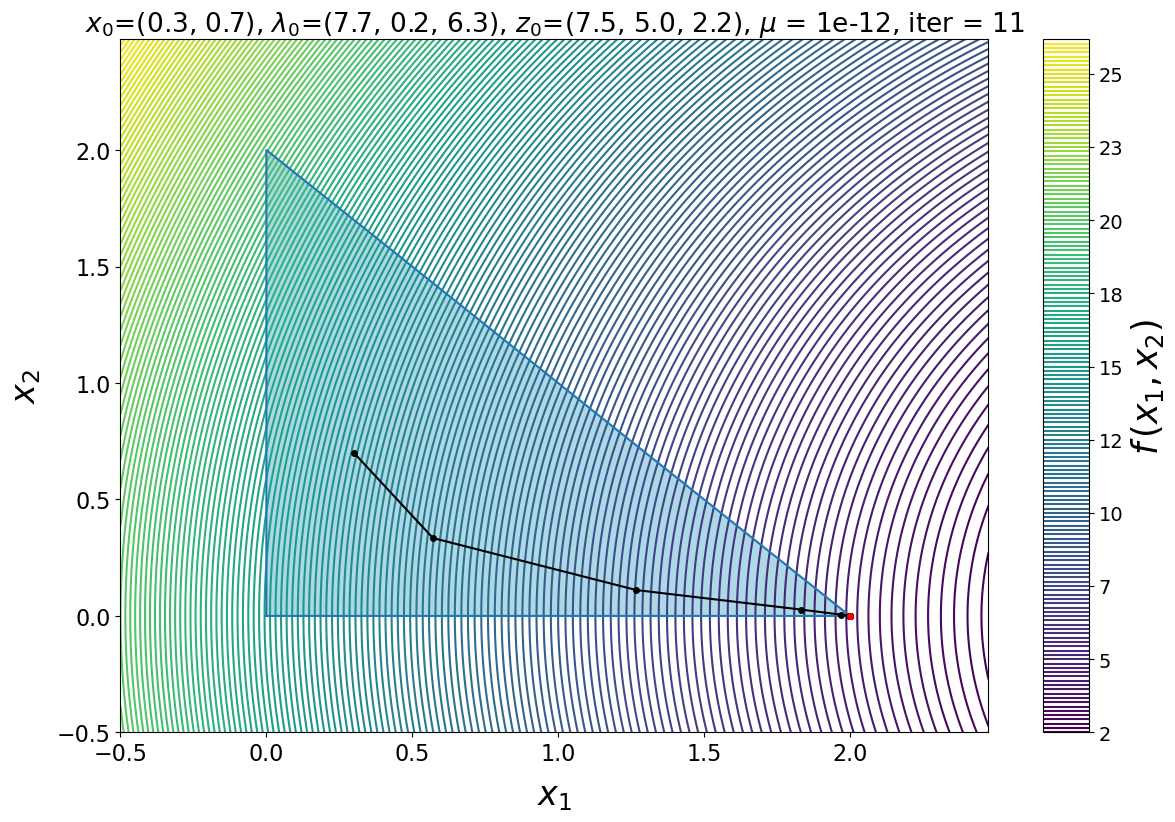
\includegraphics[scale=0.28]{Plot/func_a_method=basic_x0=[0.3 0.7]_mu=1e-12_seed=10.png}} \
	\subfloat[][]{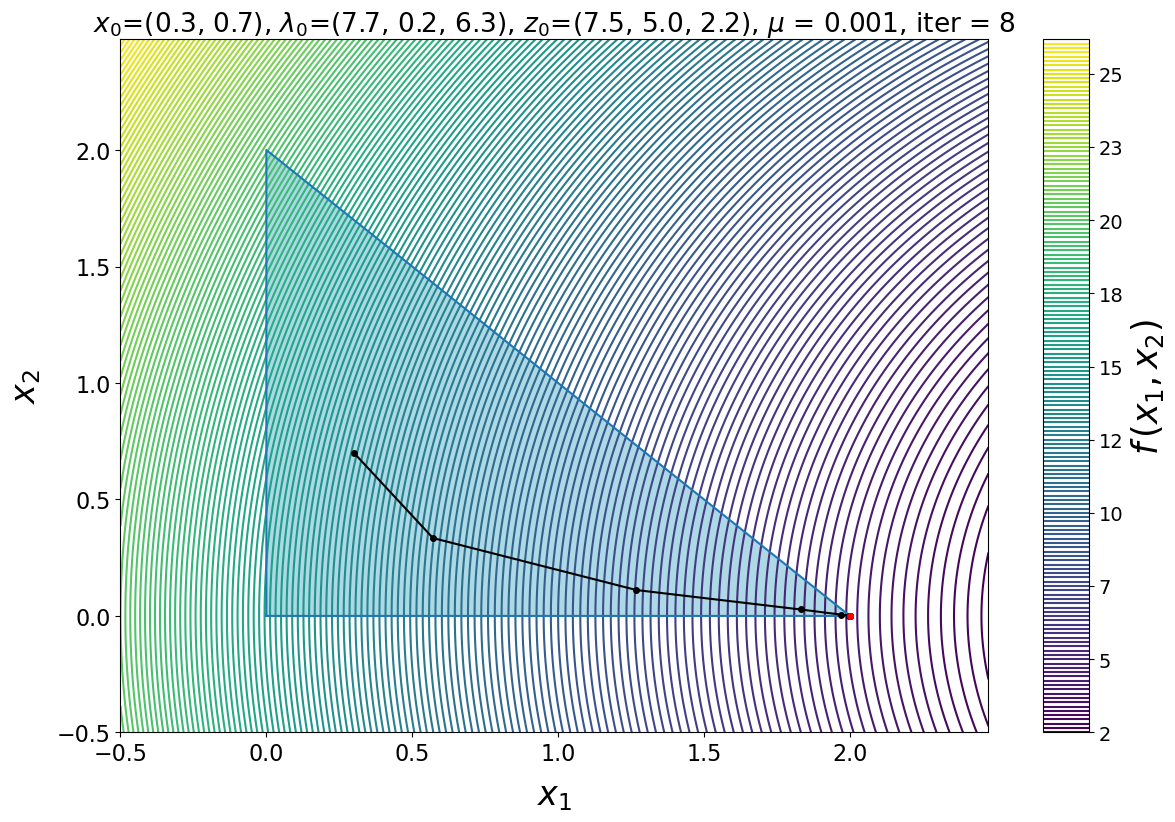
\includegraphics[scale=0.28]{Plot/func_a_method=basic_x0=[0.3 0.7]_mu=0.001_seed=10.png}}
	\caption{Contour plot of the function $f_{a}(x_{1},x_{2})$ with $\mu=10^{-12}$ (Panel (a)) and $\mu=10^{-3}$ (Panel (b)), together with the constrained set, in blue. Values of $\textbf{x}_{0}$, $\boldsymbol{\lambda}_{0}$, and $\textbf{z}_{0}$ in the titles of the plots. In red is the constrained minimum point the interior point algorithm converges to.}
	\label{Fig:func_a_diff_mu}
\end{figure}

\noindent To better compare the values of the computed minimum points and those of $\boldsymbol{\lambda}$, and $\textbf{z}$ at the final iteration, we report below the numerical results that we find in correspondence with the plots in Fig \ref{Fig:func_a_diff_mu}.\\

\begin{minted}{text}

x_0 = (0.3, 0.7), lambda_0 = (3.3, 3.6, 0.4), z_0 = (3.0, 5.8, 3.2)

mu = 1e-12, iter = 11
min point = (1.9999999999994307, 2.626380016246266e-13)
min value = 4.000000000002277
lambda_fin = (4.000000000001556, 4.174412551738449e-13, 4.000000000002081)
z_fin = (3.065889841752647e-13, 1.9999999999994307, 2.626387608486303e-13)

mu = 0.001, iter = 8
min point = (1.9995002185977582, 0.0002498750975605184)
min value = 4.001999437827982
lambda_fin = (4.0014996877813, 0.0005001249768169601, 4.001999437976421)
z_fin = (0.0002499063046813427, 1.9995002185977582, 0.0002498750975605184)
\end{minted}

\noindent As we can see from these results, in both cases the algorithm converges to the exact minimum point $\textbf{x}^*=(2,0)^{T}$ and to the vectors $\boldsymbol{\lambda}^*=(4,0,4)^{T}$ and $\textbf{z}^*=(0,2,0)^{T}$, with an error that is of $\mathcal{O}(\mu)$ and with a number of steps which decreases as $\mu$ increases.
%We can also note that $\textbf{z}^*=(0,2,0)^{T}$ is compatible, within this error, with the value of the function $\textbf{c}(\textbf{x})$ at the computed minimum point.
We can also note that the computed value of the slack variable is compatible, within this error, with the value of the function $\textbf{c}_{a}(\textbf{x})$ at $\textbf{x}^*$.\\

\noindent Finally, for the same triad of vectors, we report a plot with the number of iterations until convergence as a function of $\log_{10}(\mu)$.
\begin{figure}[H]
	\centering
	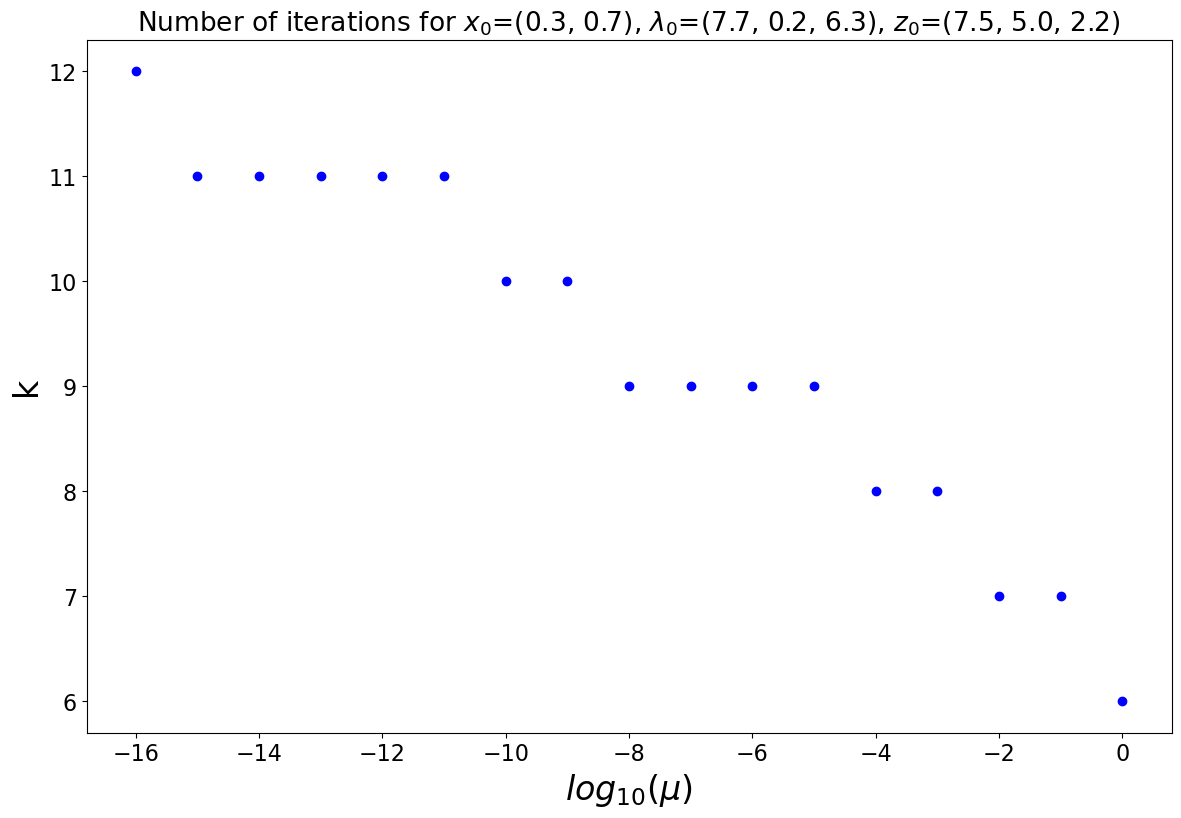
\includegraphics[scale=0.35]{Plot/number_iter_method=basic_x0=[0.3 0.7]_seed=10.png}
	\caption{Scatter plot of the number of iterations until convergence as a function of $\log_{10}(\mu)$, for the triad of vectors $\textbf{x}_{0}$, $\boldsymbol{\lambda}_{0}$, and $\textbf{z}_{0}$ reported in the title of the plot.}
	\label{Fig:func_a_number_iter}
\end{figure}
%Therefore, as expected, when increasing the value of $\mu$ the algorithm converges to a less precise solution with fewer steps.
%
%
%\noindent As we can see from these results, for $\mu=10^{-12}$ the algorithm returns a constrained minimum point that is much closer to the exact value with respect to the case with $\mu=10^{-3}$, and the same holds for the values of $\boldsymbol{\lambda}^*$ and $\textbf{z}^*$ which are, respectively, the vector of Lagrange multipliers and the vector of slack variables computed in correspondence with the minimum point. In general, we can observe that the error on these values is of $\mathcal{O}(\mu)$.
%
%We can note that, within this error, the algorithm converges in both cases to the exact minimum point $\textbf{x}^*=(2,0)^{T}$ and to $\boldsymbol{\lambda}^*=(4,0,4)^{T}$, which are solutions to the KKT system. Moreover, we also find $\textbf{z}^*=(0,2,0)^{T}$, which is compatible, within the same error, with $\textbf{c}(\textbf{x}^*)$.\\ 

\noindent For demonstration purposes, we report in the following other convergence paths emerging when considering different initial points and different values of $\boldsymbol{\lambda}_{0}$ and $\textbf{z}_{0}$. In this case, we fixed $\mu=10^{-12}$.
\begin{figure}[H]
	\centering
	\subfloat[][]{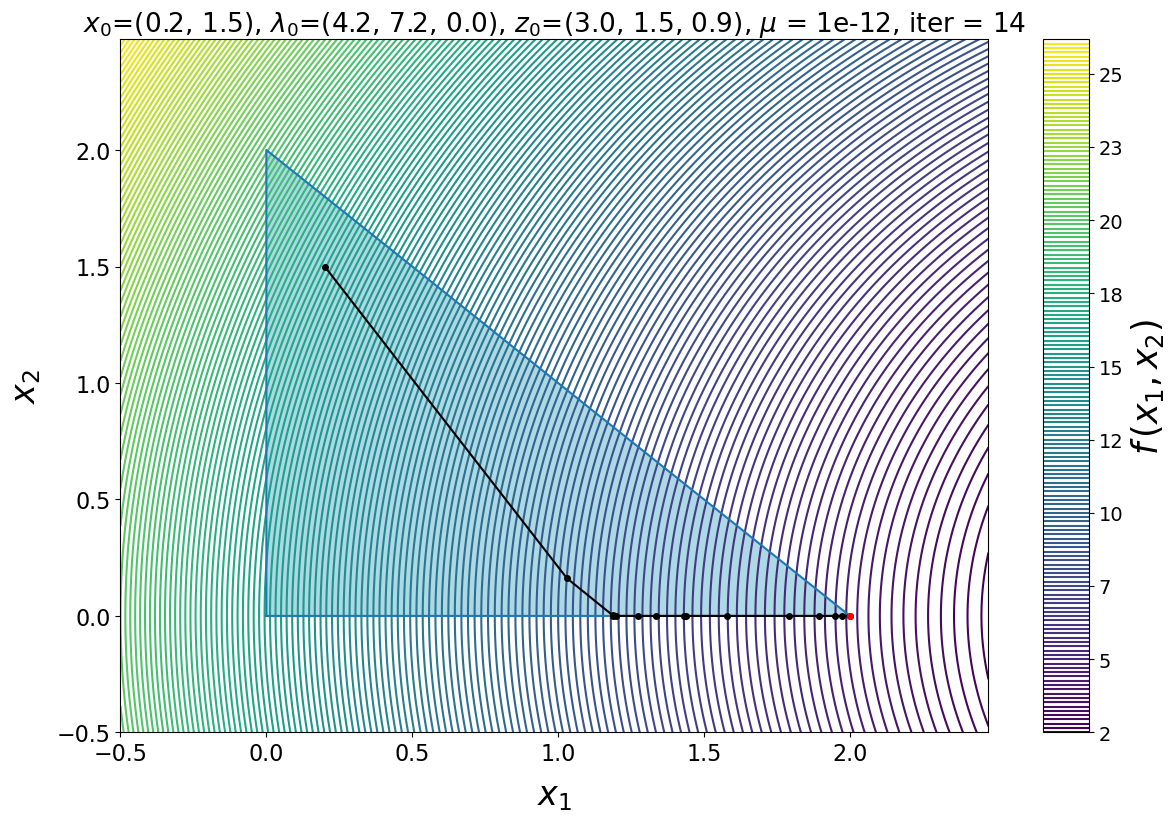
\includegraphics[scale=0.28]{Plot/func_a_method=basic_x0=[0.2 1.5]_mu=1e-12_seed=1.png}} \
	\subfloat[][]{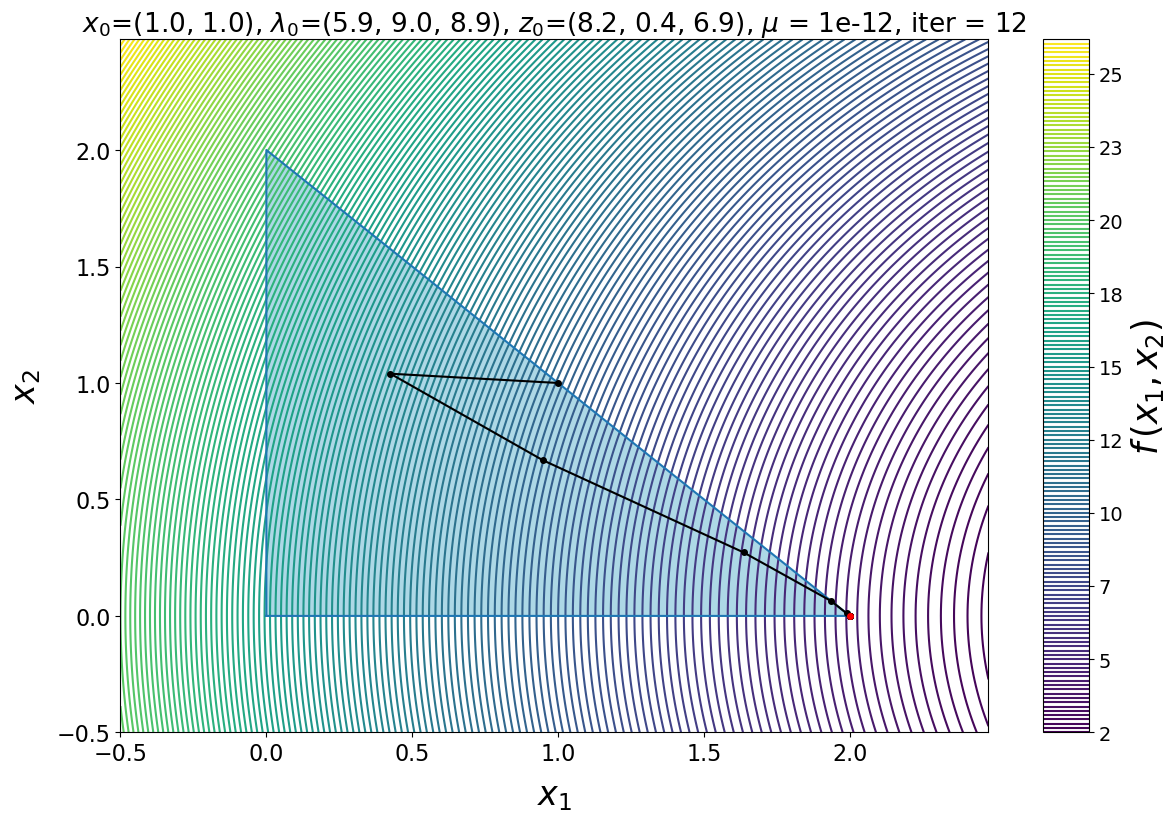
\includegraphics[scale=0.28]{Plot/func_a_method=basic_x0=[1. 1.]_mu=1e-12_seed=20.png}}
	\caption{Contour plot of the function $f_{a}(x_{1},x_{2})$ with $\mu=10^{-12}$ and different values of $\textbf{x}_{0}$, $\boldsymbol{\lambda}_{0}$, and $\textbf{z}_{0}$, reported in the title of the plots. The constrained set is represented by the triangle in blue. In red is the constrained minimum point the interior point algorithm converges to.}
	\label{Fig:func_a_diff_x0}
\end{figure}

\subsection*{Function $\boldmath{f_{b}}(\textbf{x})$}
In this case, from the previous analysis, we know that the KKT system has two solutions, namely $\textbf{x}^*_{1}=(0,1)$, with $\boldsymbol{\lambda}_{1}^*=(1,2,0)$, and $\textbf{x}^*_{2}=(0,0)$, with $\boldsymbol{\lambda}_{2}^*=(0,2,0)$. Given that $f_{b}(\textbf{x}_{1}^*) = -1$ and $f_{b}(\textbf{x}_{2}^*) = 0$, we know that $\textbf{x}^*_{1}=(0,1)$ is the unique constrained minimum of this problem. In this case, we expect that the interior point algorithm may not always converge to the point $\textbf{x}^*_{1}$ but, sometimes, depending on the values of the input vectors $\textbf{x}_{0}$, $\boldsymbol{\lambda}_{0}$, and $\textbf{z}_{0}$, it may also converge to the point $\textbf{x}^*_{2}$.\\

\noindent In order to study this problem, we use the method \mintinline{Python}{'basic'}, which solves the complete linear system to compute the Newton step, and we set the variable \mintinline{Python}{curv = True}, so to consider the curvature term in the expression of the Jacobian of the problem, since, in this case, the constraints are quadratic in $x_{1},x_{2}$.\\

\noindent We report in the Fig.~\ref{Fig:func_b_diff_x0} the plots of the convergence paths toward the point $\textbf{x}^*_{1}$ that we find when considering different initial values of $\textbf{x}_{0}$, $\boldsymbol{\lambda}_{0}$, and $\textbf{z}_{0}$, while fixing $\mu=10^{-12}$. Below are the numerical results that we obtain for the first one of the four cases analyzed.
\begin{minted}{text}
convergence = True, with 19 steps and method = basic
starting point = (0.5, 0.5)
mu = 1e-12, lambda_0 = (1.5, 7.4, 2.6), z_0 = (5.3, 0.1, 9.2)        
min point = (5.000000371825291e-13, 0.9999999999995)
min value = -0.9999999999979999
lambda_fin = (1.0000000000005, 2.000000000001, 9.999941060547193e-13)   
z_fin = (1.0000141425515907e-12, 5.000000371767508e-13, 0.9999999999995)
\end{minted}

\noindent We can note that the algorithm converges to the vectors $\textbf{x}_{1}^*$, $\boldsymbol{\lambda}_{1}^*$, and $\textbf{z}_{1}^* \coloneqq \textbf{c}_{b}(\textbf{x}_{1}^*)$, within an error of $\mathcal{O}(\mu)$. The same hold for the other three considered cases in Fig. \ref{Fig:func_b_diff_x0}, not reported here.
\begin{figure}[H]
	\centering
	\subfloat[\label{fig:func_b_05_05}]{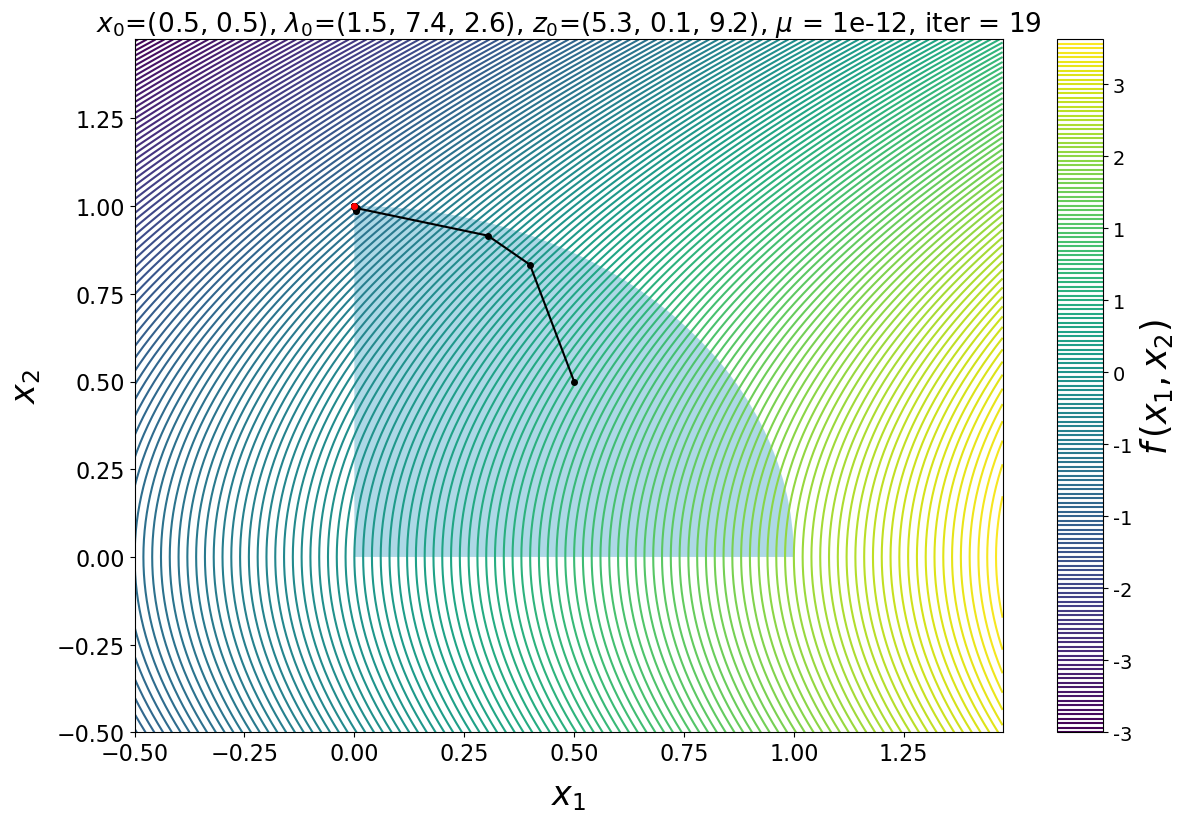
\includegraphics[scale=0.28]{Plot/func_b/contourplot/func_b_method=basic_x0=[0.5 0.5]_mu=1e-12_seed=12}} \
	\subfloat[\label{fig:func_b_07_03}]{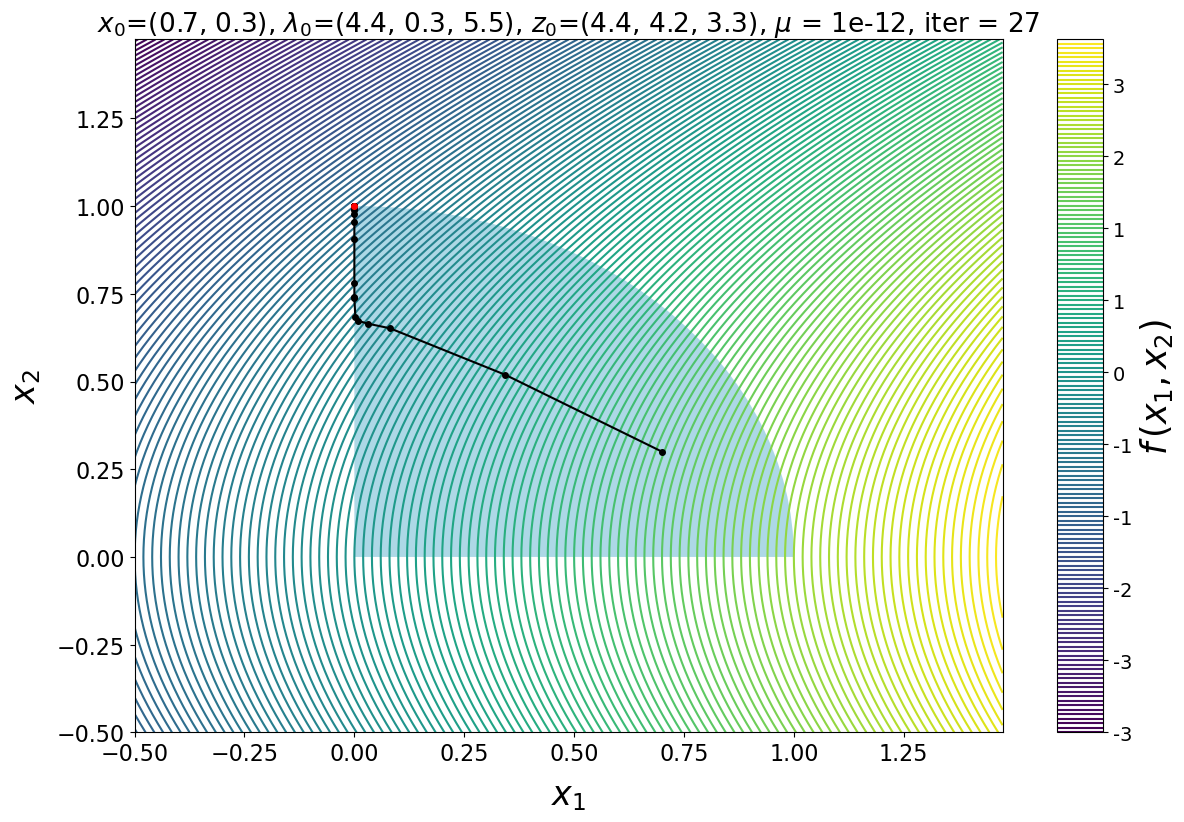
\includegraphics[scale=0.28]{Plot/func_b/contourplot/func_b_method=basic_x0=[0.7 0.3]_mu=1e-12_seed=2}} \\
	\subfloat[\label{fig:func_b_09_01}]{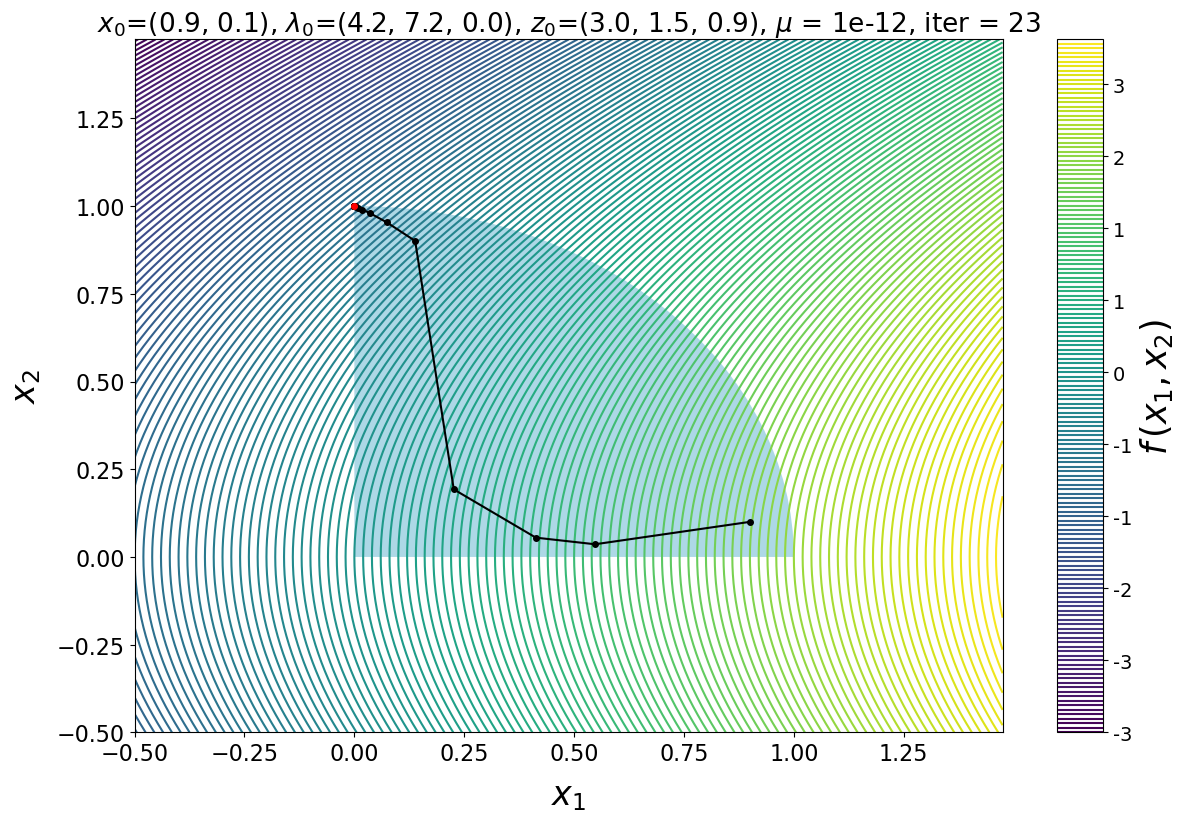
\includegraphics[scale=0.28]{Plot/func_b/contourplot/func_b_method=basic_x0=[0.9 0.1]_mu=1e-12_seed=1.png}} \
	\subfloat[\label{fig:func_b_02_06}]{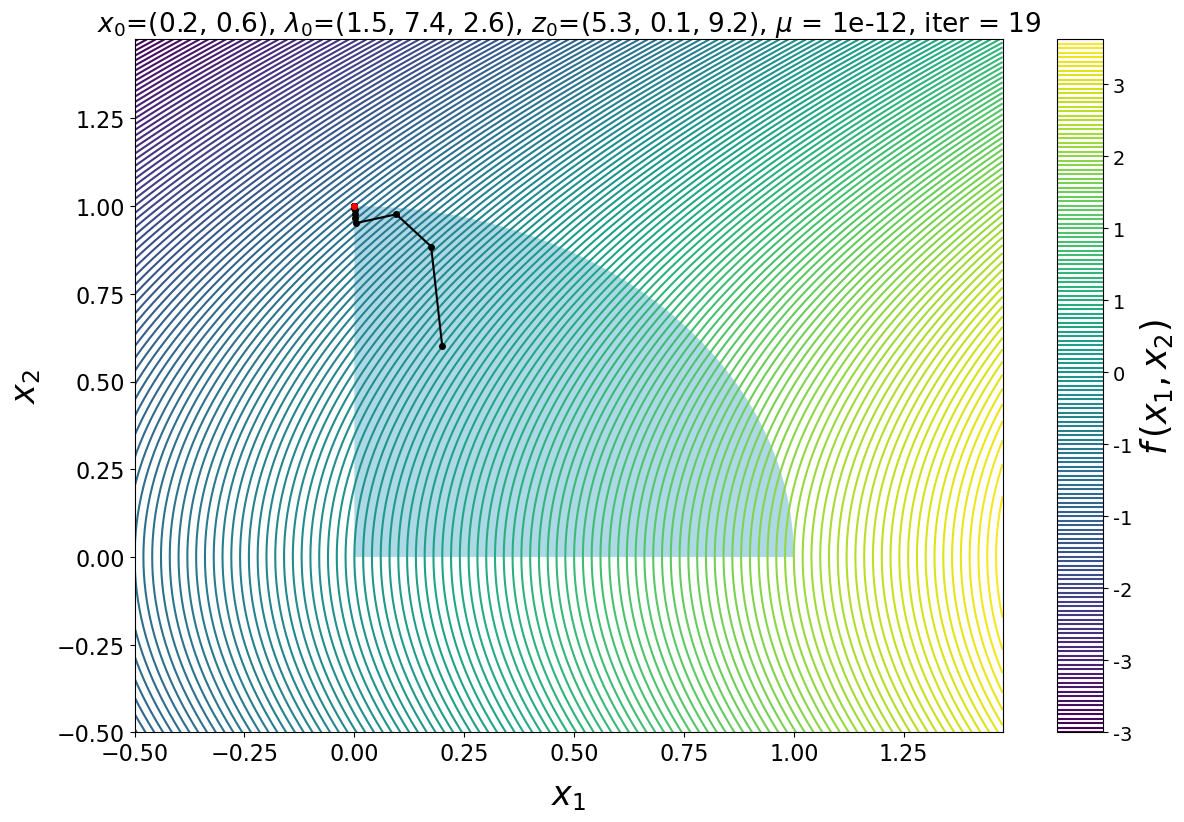
\includegraphics[scale=0.28]{Plot/func_b/contourplot/func_b_method=basic_x0=[0.2 0.6]_mu=1e-12_seed=12}}
	\caption{Contour plot of the function $f_{b}(x_{1},x_{2})$ with $\mu=10^{-12}$ and different values of $\textbf{x}_{0}$, $\boldsymbol{\lambda}_{0}$, and $\textbf{z}_{0}$, reported in the title of the plots. The constrained set is represented in blue. In red is the constrained minimum point the interior point algorithm converges to.}
	\label{Fig:func_b_diff_x0}
\end{figure}
\noindent As we can see from these plots, in all these cases, the algorithm converges to the right constrained minimum $\textbf{x}_{1}^*=(0,1)$. However, we also observe situations in which the algorithm, stops at the point $\textbf{x}_{2}^*=(0,0)$ with $\boldsymbol{\lambda}_{2}^*=(0,2,0)$ and $\textbf{z}_{2}^*=(1,0,0)$, which is the other solution of the KKT system. We report, as an example, the numerical results that we obtain for the first one of the two cases in Fig. \ref{Fig:func_b_diff_x0_non_conv}, where this behavior is observed.
\begin{minted}{text}
convergence = False, with 100 steps and method = basic
starting point = (0.1, 0.1)
mu = 1e-12, lambda_0 = (7.7, 0.2, 6.3), z_0 = (7.5, 5.0, 2.2)
min point = (5e-13, 5.717234610811308e-07)
min value = 6.731322840494127e-13
lambda_fin = (9.999999999948479e-13, 2.0, 1.2049499133358223e-06)
z_fin = (1.0000000000019542, 5e-13, 5.717234610811308e-07)
\end{minted}




\begin{figure}[H]
	\centering
	\subfloat[\label{fig:func_b_01_01}]{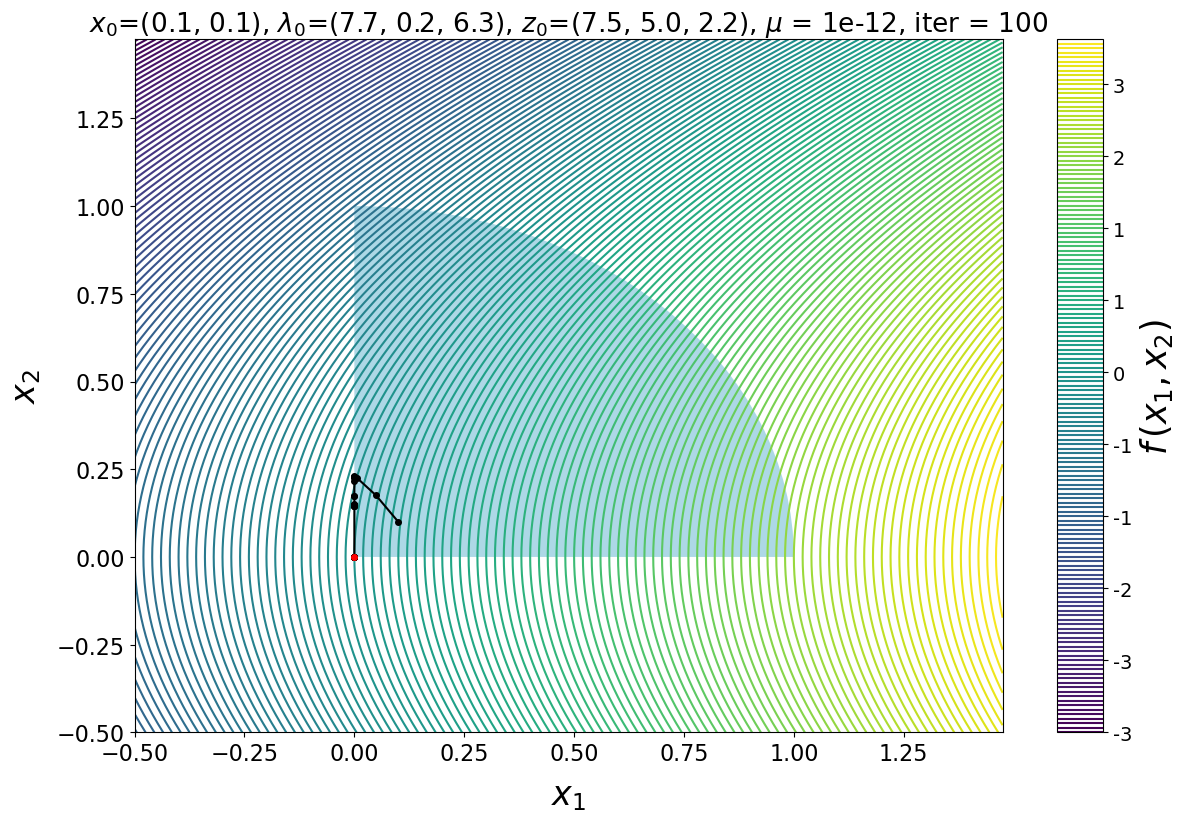
\includegraphics[scale=0.28]{Plot/func_b/contourplot/func_b_method=basic_x0=[0.1 0.1]_mu=1e-12_seed=10}} \
	\subfloat[\label{fig:func_b_025_025}]{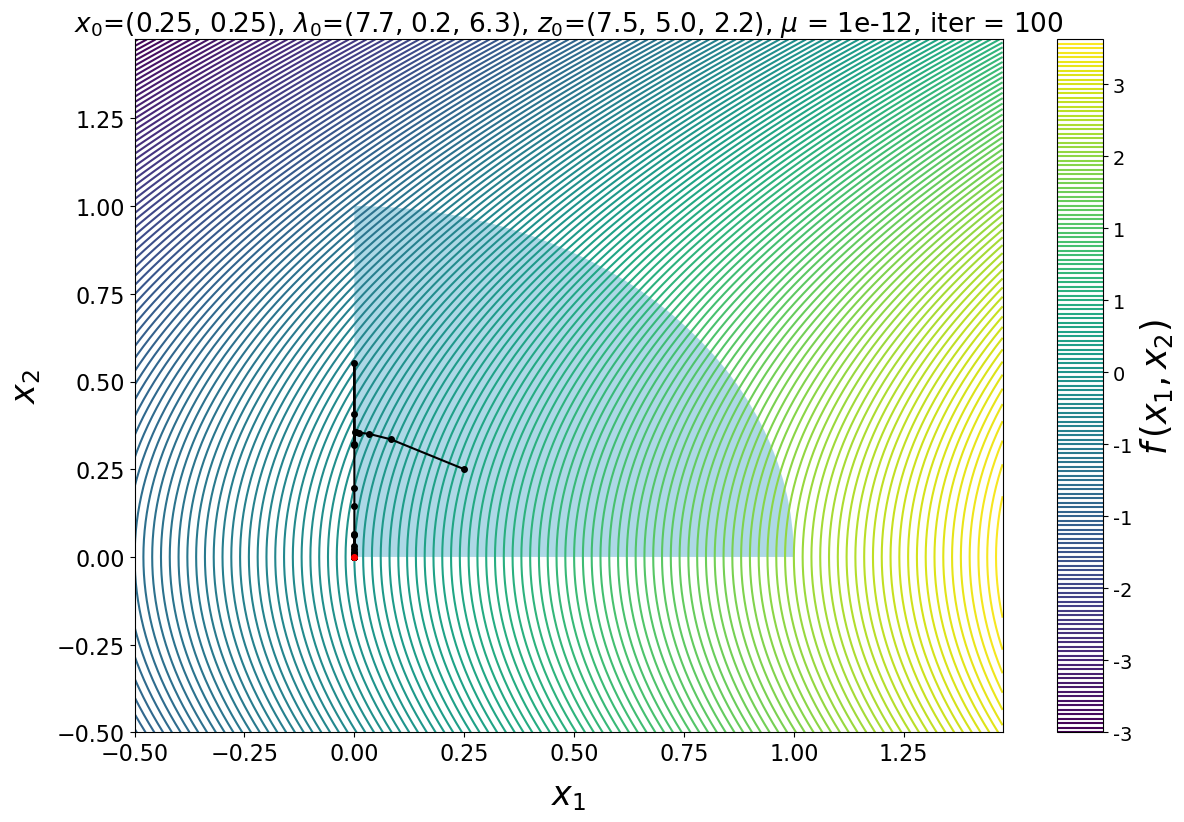
\includegraphics[scale=0.28]{Plot/func_b/contourplot/func_b_method=basic_x0=[0.25 0.25]_mu=1e-12_seed=10}} \\
	\caption{Contour plot of the function $f_{b}(x_{1},x_{2})$ with $\mu=10^{-12}$ and different values of $\textbf{x}_{0}$, $\boldsymbol{\lambda}_{0}$, and $\textbf{z}_{0}$, reported in the title of the plots. The constrained set is represented in blue. In red is the constrained minimum point the interior point algorithm converges to.}
	\label{Fig:func_b_diff_x0_non_conv}
\end{figure}

\noindent Since in this case the KKT system has two solutions and the dependence of the convergence of the algorithm from the initial parameters is expected to be stronger than in the previous case, we have decided to deepen how this convergence depends on $\boldsymbol{\lambda}_{0}$ and $\textbf{z}_{0}$.
In order to do it, we have chosen two representative initial points, namely $(0.5,0.5)$ and $(0.1,0.1)$.
For the considered values of $\boldsymbol{\lambda}_{0}$ and $\textbf{z}_{0}$, we have found that for the first point the algorithm converges to $\textbf{x}_{1}^*$, which is the right minimum point, while, for the second one, the algorithm does not converge and it arrives to $\textbf{x}_{2}^*$ after the maximum number of iterations allowed (see Fig. \ref{fig:func_b_05_05}, \ref{fig:func_b_01_01}). However, since $\boldsymbol{\lambda}_{0}$ and $\textbf{z}_{0}$ can be chosen randomly, to simplify this analysis we have decided to consider vectors of the form $\boldsymbol{\lambda}_{0}=\lambda(1,1,1)$, $\textbf{z}_{0}=z(1,1,1)$ and we have varied $\lambda$ and $z$ in the range $[10^{-12},10]$, with a step of $0.1$. For each couple $(\lambda,z)$, we have run the algorithm, both considering the curvature term and not considering it, and we have stored the number of iterations performed.
%Finally, we have plotted the results in a colorplot.\\
%\noindent Note that there are three possible situations that can appear:
%\begin{enumerate}
%	\item the algorithm converges to the right minimum point $\textbf{x}_{1}^*$;
%	\item the algorithm converges to the point $\textbf{x}_{2}^*$, solution of the KKT system;
%	\item the algorithm does not converge within the maximum number ($100$) of iterations allowed.
%\end{enumerate}
%To distinguish these three cases, we have manually assigned to $k$ the value $k=150$ when the algorithm converges to a point $\tilde{\textbf{x}}$ such that $\| \tilde{\textbf{x}} - \textbf{x}_{2}^*  \|_{2} < 10^{-2}$.\\
%
Finally, to distinguish when the algorithm arrives at the point $\textbf{x}_{2}^*$, we have manually assigned to $k$ the value $k=150$ when the algorithm stops at a point $\tilde{\textbf{x}}$ such that $\| \tilde{\textbf{x}} - \textbf{x}_{2}^*  \|_{2} < 10^{-2}$.\\

\noindent We report in Fig. \ref{Fig:func_b_colorplot} the obtained results.
\begin{figure}[H]
	\centering
	\subfloat[][]{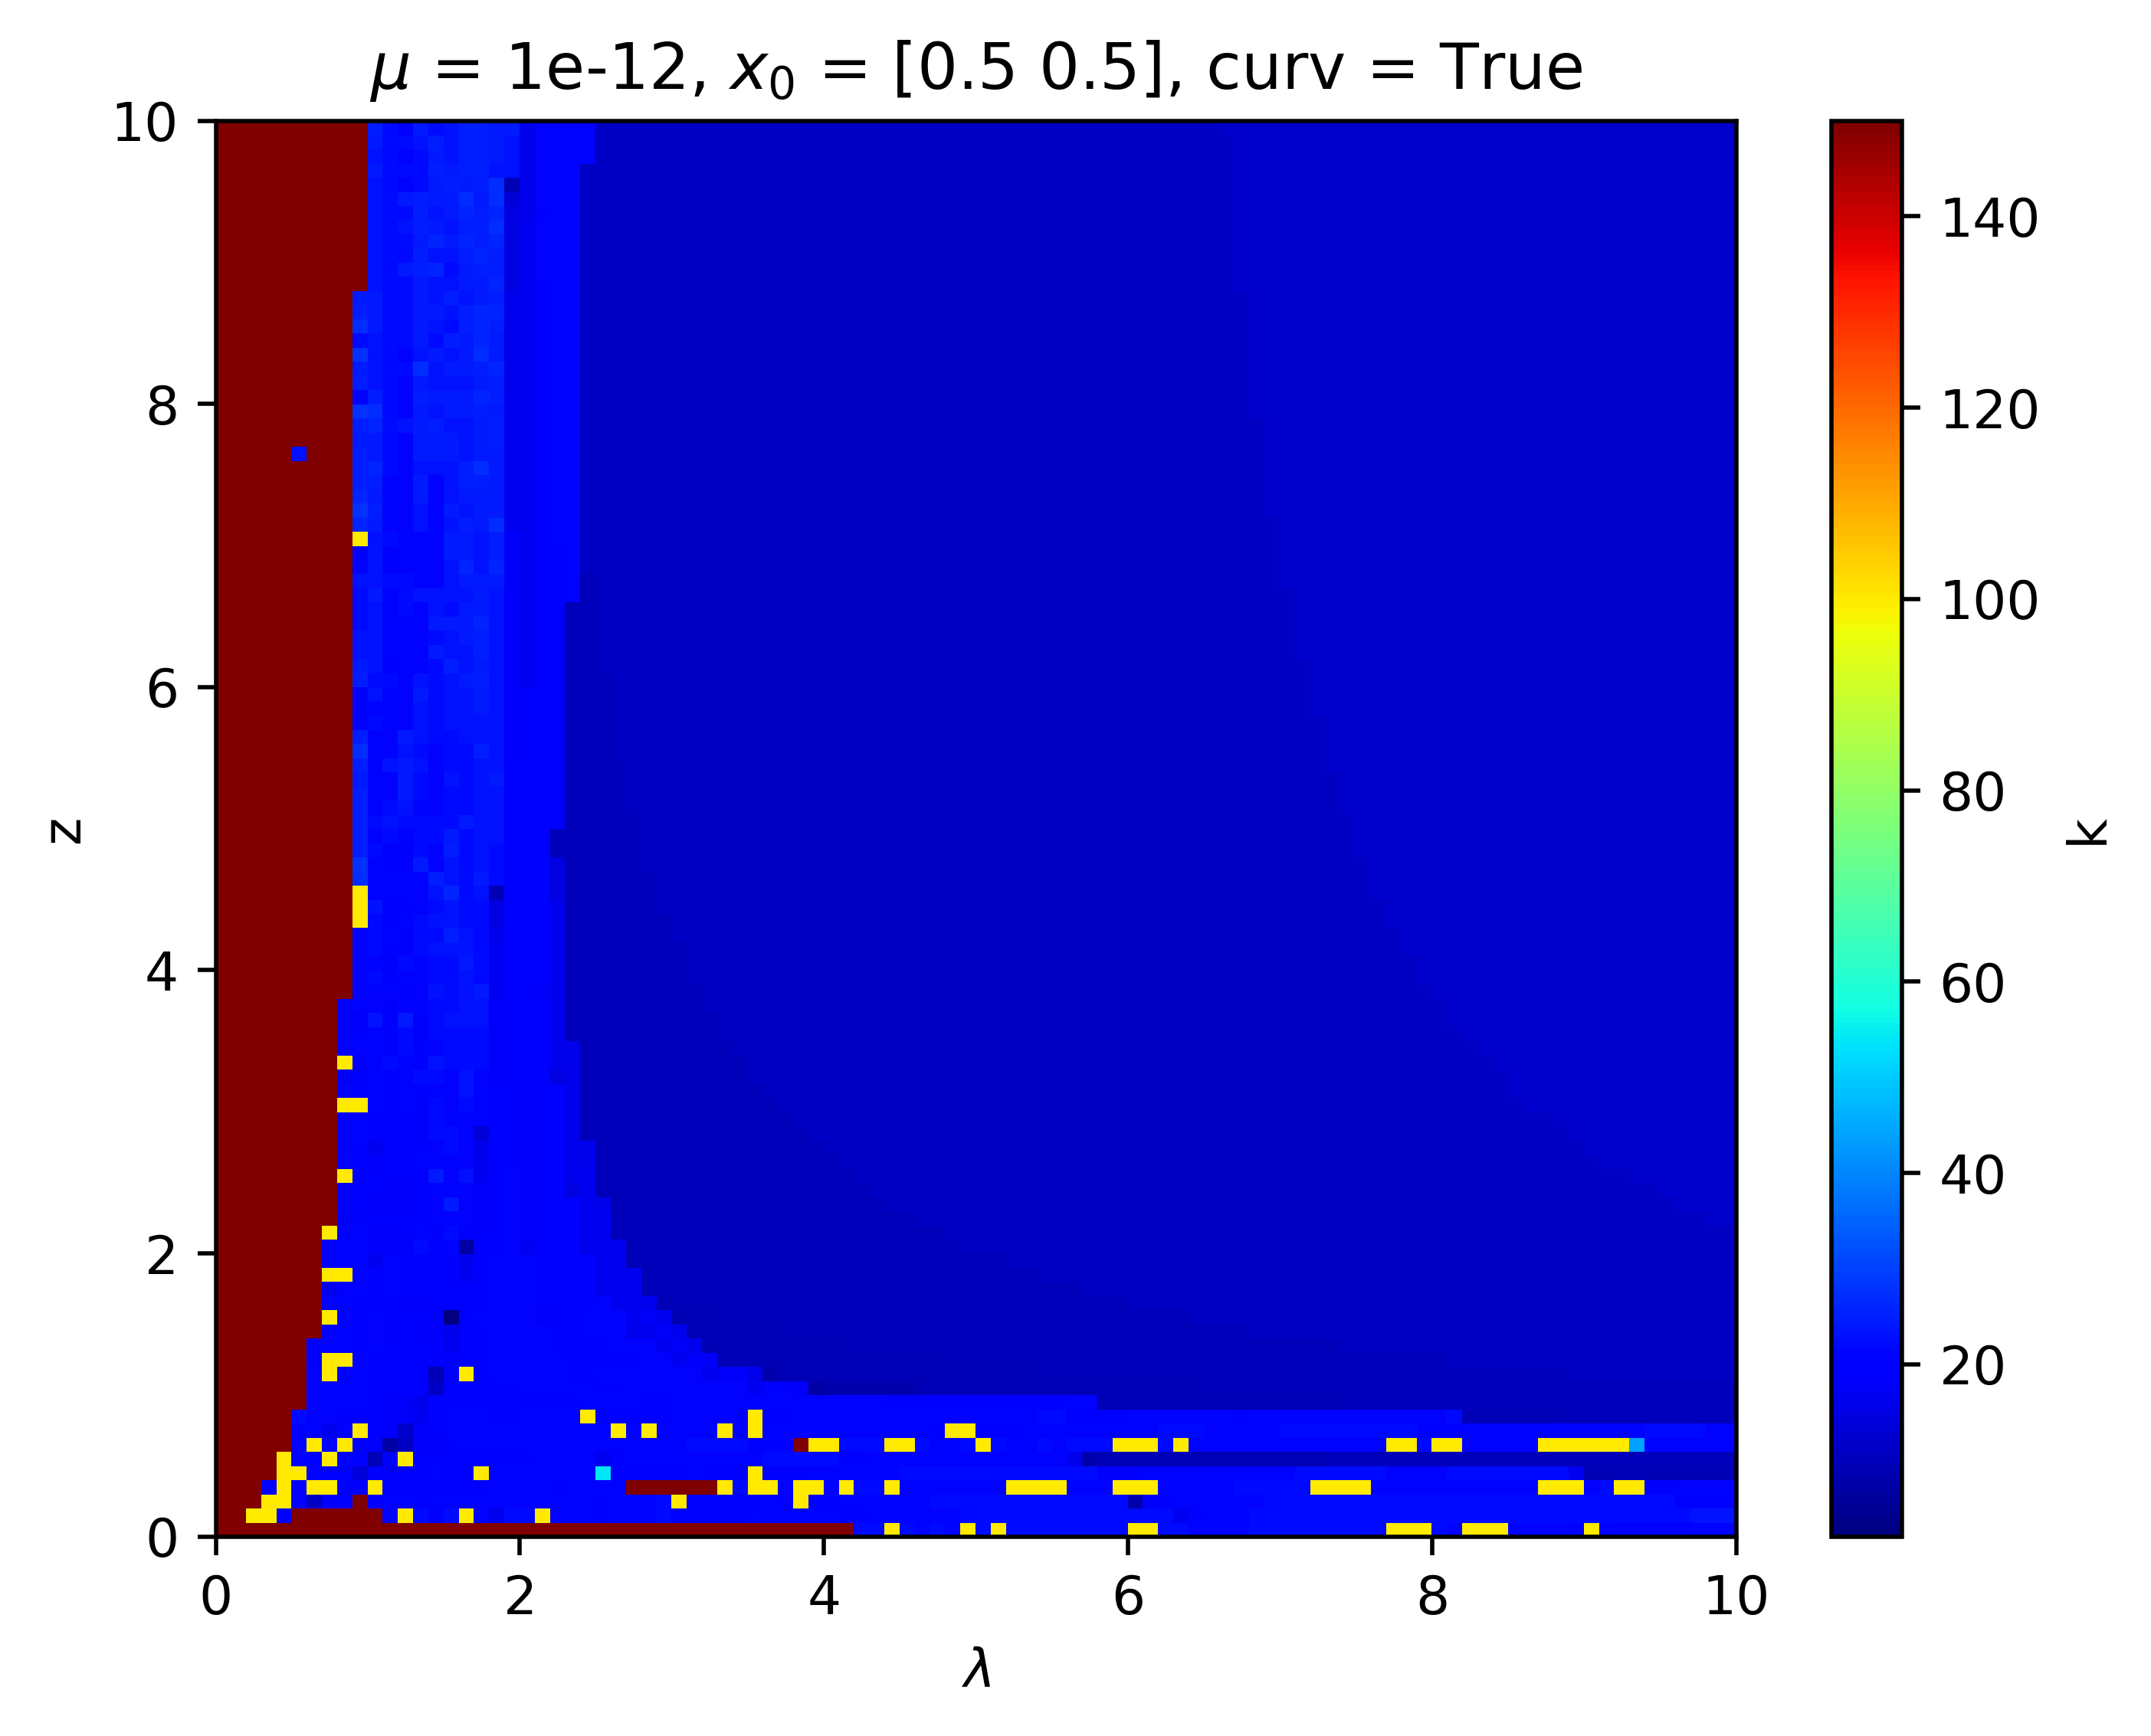
\includegraphics[scale=0.55]{Plot/func_b/colorplot/func_b_with_K_method=basic_x0=[0.5 0.5]_mu=1e-12_tol=0.010000000001}} \
	\subfloat[][]{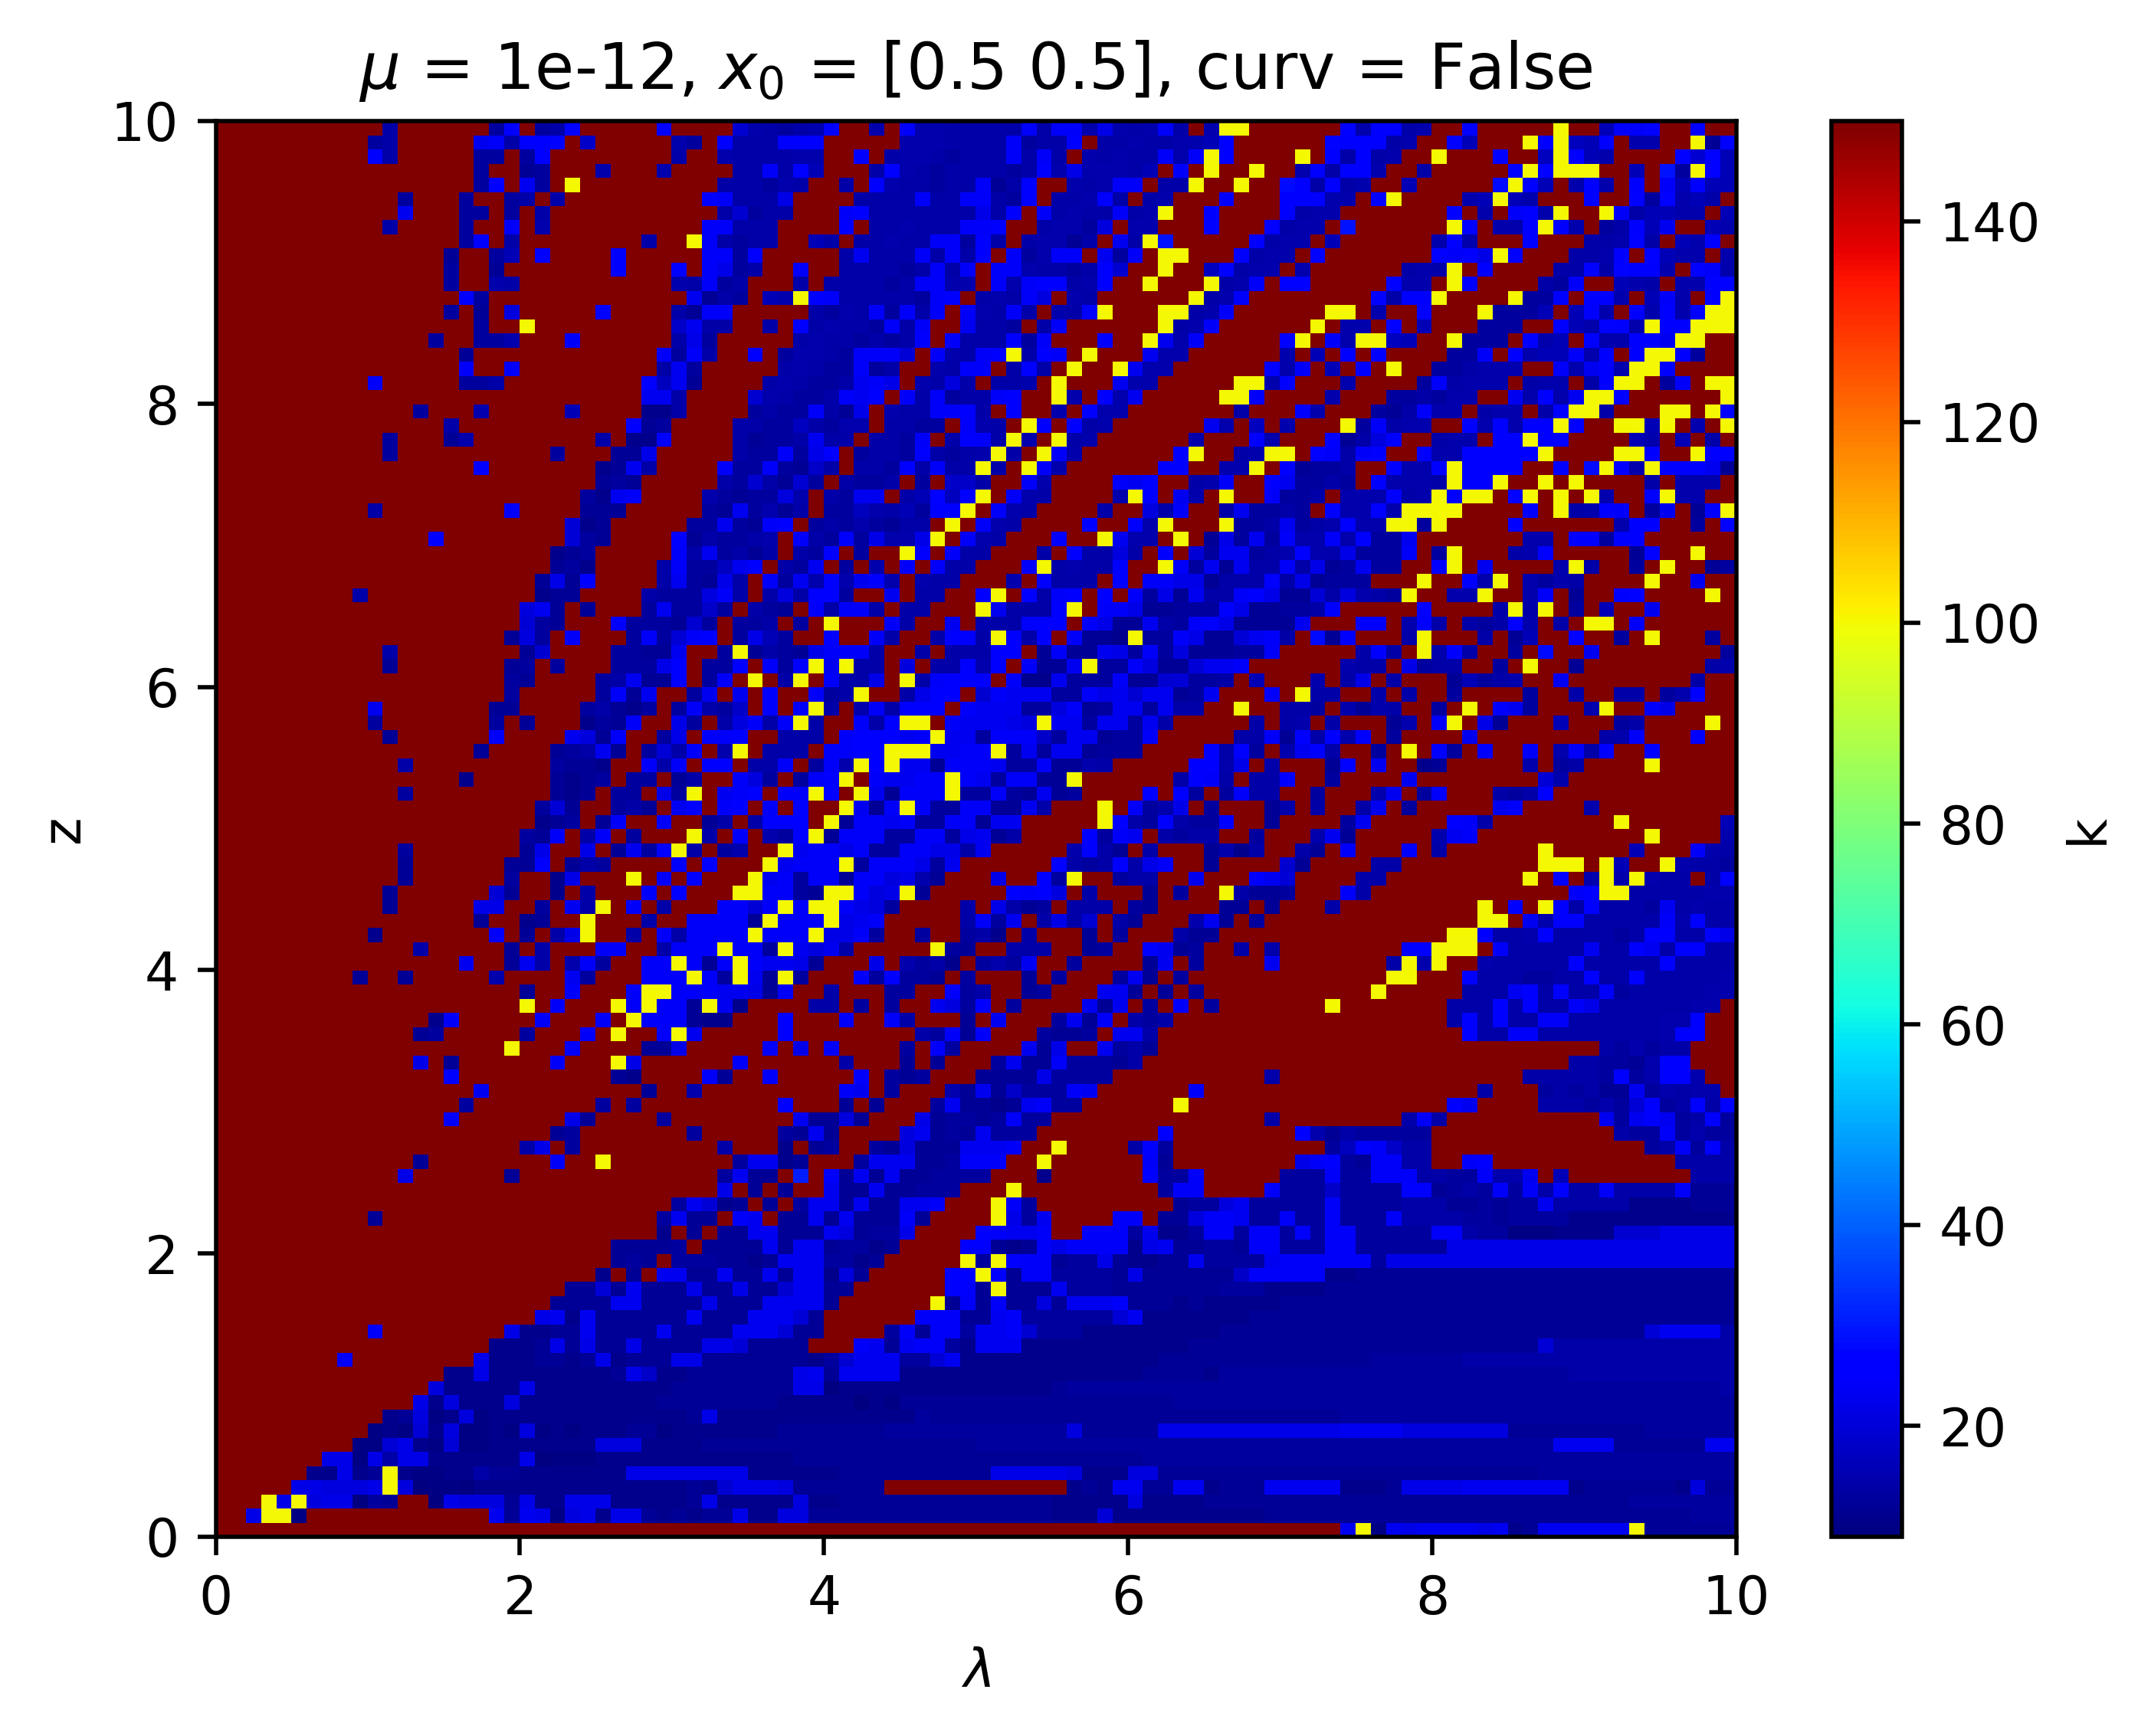
\includegraphics[scale=0.55]{Plot/func_b/colorplot/func_b_method=basic_x0=[0.5 0.5]_mu=1e-12_tol=0.010000000001}} \\
	\subfloat[][]{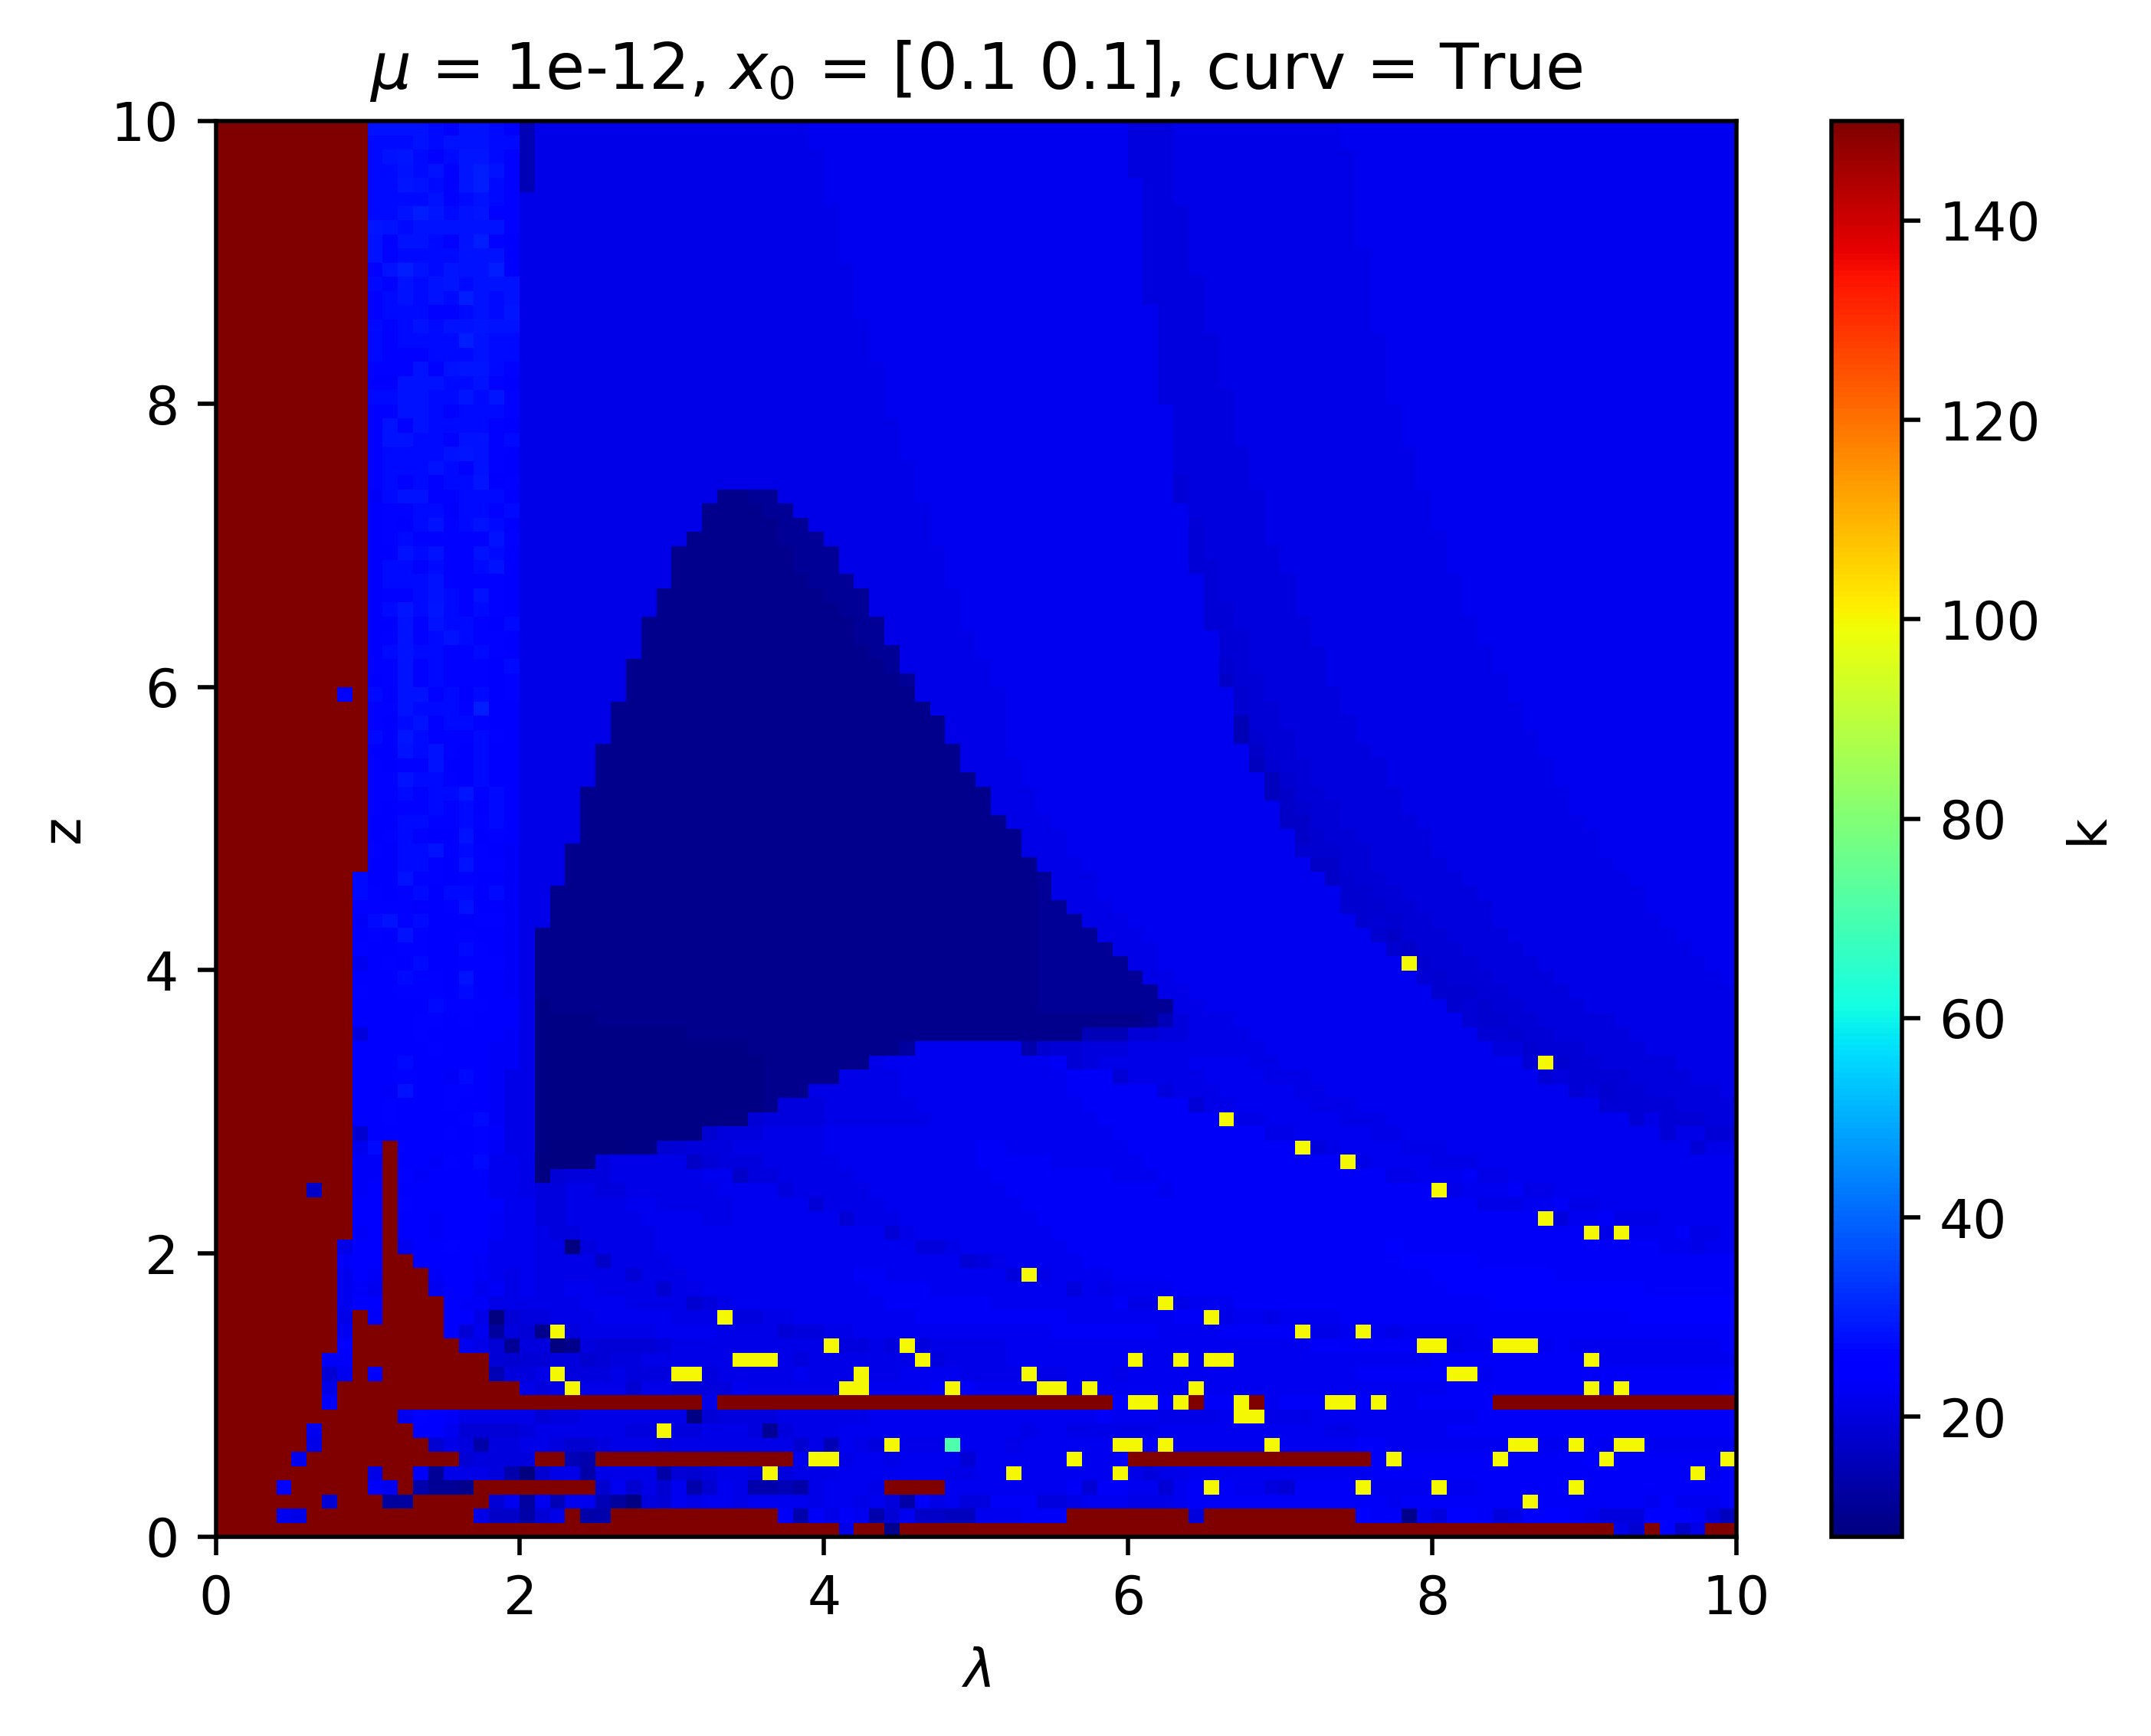
\includegraphics[scale=0.55]{Plot/func_b/colorplot/func_b_with_K_method=basic_x0=[0.1 0.1]_mu=1e-12_tol=0.010000000001}} \
	\subfloat[][]{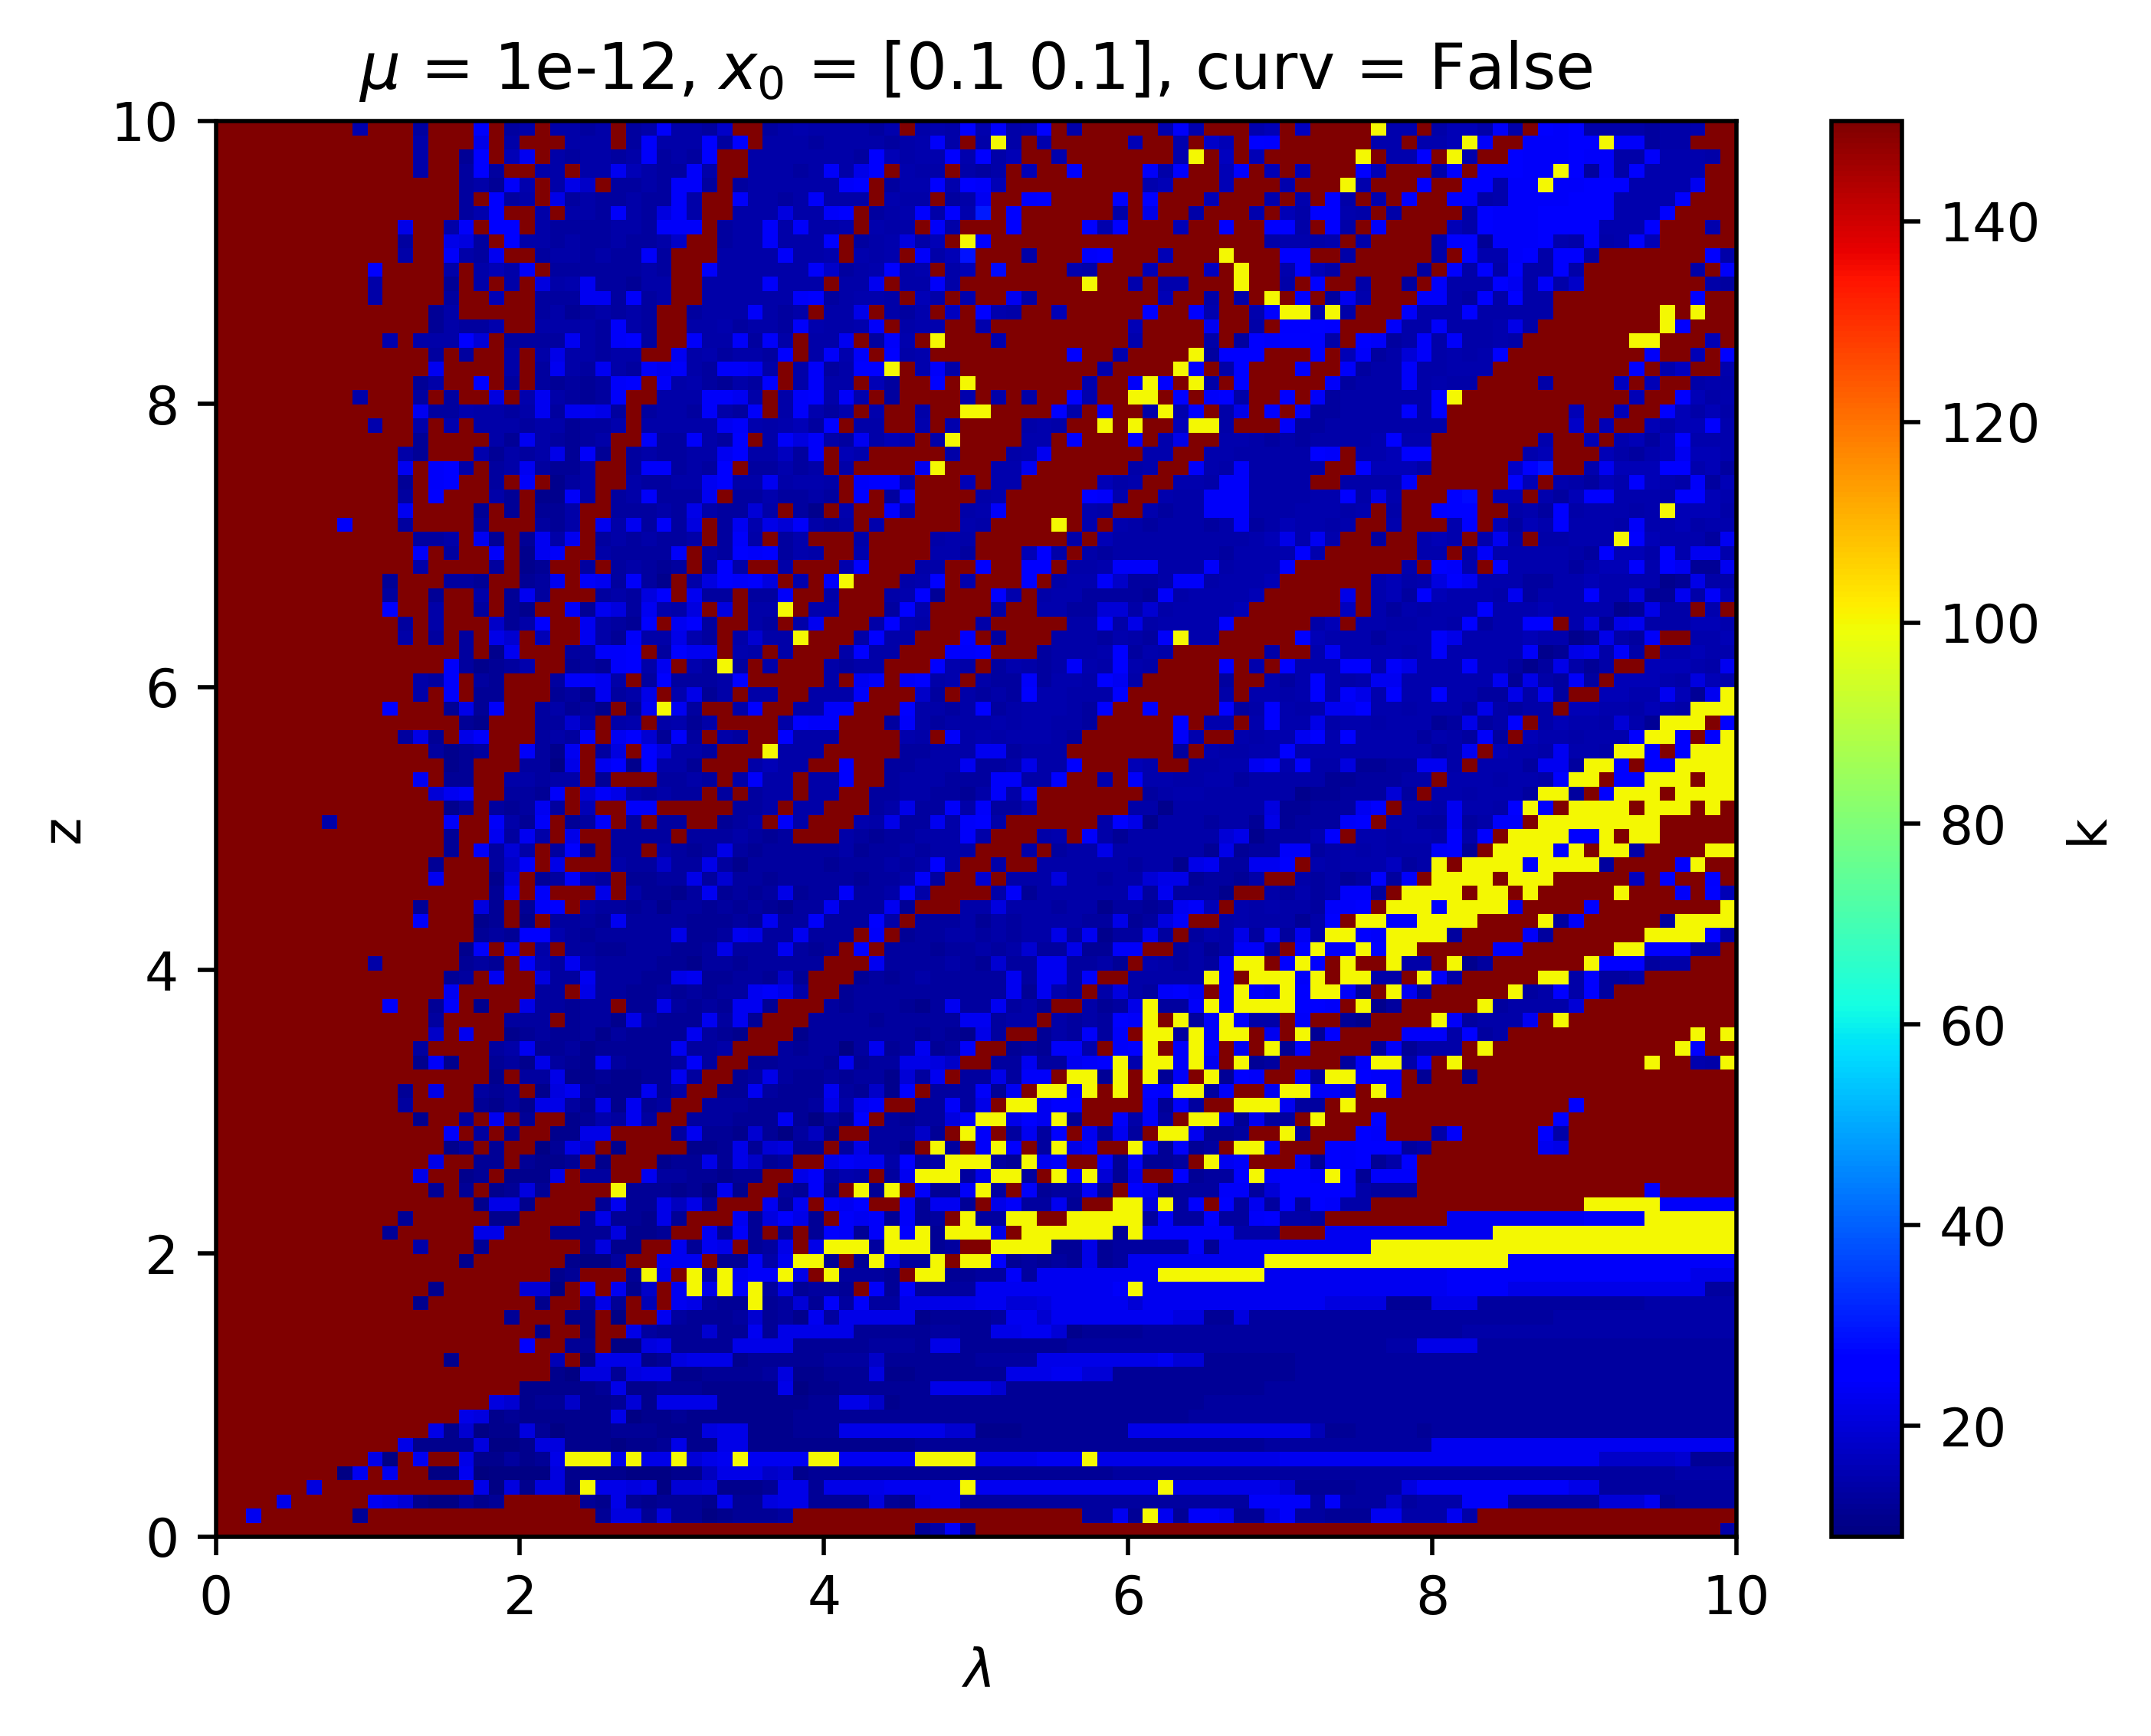
\includegraphics[scale=0.55]{Plot/func_b/colorplot/func_b_method=basic_x0=[0.1 0.1]_mu=1e-12_tol=0.010000000001}} \\
	\caption{Colorplot of the number of iterations until convergence for the function $f_{b}(\textbf{x})$, with $\mu=10^{-12}$ and different values of $\textbf{x}_{0}$, reported in the title of the plots. The parameter curv = True indicates the presence of the curvature term in the expression of the Jacobian of the system.}
	\label{Fig:func_b_colorplot}
\end{figure}

\noindent The first thing that emerges from these plots is that the addition of the curvature term strongly improves the convergence of the algorithm to the right minimum point. This is expected since the constraint functions are quadratic in $x_{1},x_{2}$.  Moreover, for the chosen tolerance parameter and the maximum number of iterations allowed, we can also observe that, most of the times, when the algorithm does not converge to $\textbf{x}_{1}^*$, it stops in the neighborhood of the other solution of the KKT system, namely $\textbf{x}_{2}^*$, while there are few points (in yellow) where the algorithm does not converge either to $\textbf{x}_{1}^*$ or to $\textbf{x}_{2}^*$. 

%
%
%	
%In this project we would like to find the constrained minima of some test functions first analytically, by using the KKT theorem, and then numerically, by implementing the interior point method, using Python as programming language. 
%This report will be divided into two sections. In the first one we will report the code that we have used to find numerically the minimum points of the given functions. This code can be also found in the library ***Project\_5.py*** at the following link on GitHub. In the second section, we will consider the test functions and we will report the results found both analytically and numerically.
%
%\section{Algorithm}
%
%
%\section{Test functions}
%
%\subsection{Test function (a)}
%
%We would like to minimize of the function
%\begin{equation}
%	f(x_{1},x_{2}) = (x_{1}-4)^2 + x_{2}^{2}
%	\label{eq:func_a}
%\end{equation}
%subject to the constraints
%\begin{equation}
%	x_{1} + x_{2} \le 2, \quad x_{1} \ge 0, \quad x_{2} \ge 0.
%	\label{eq:constr_a}
%\end{equation}
%
%Since the function $f(x_{1},x_{2}) = f_{1}(x_{1}) + f_{2}(x_{2}) $, reported in Eq. \eqref{eq:func_a}, is convex and positive, as it is given by the sum of two independent and positive terms, it is possible to find its unique minimum by minimizing the two adding terms separately. In other words, the second term, namely $x^{2}$, is minimized for $x_{2}=0$, while the first one, namely $(x_{1}-4)^{2}$ is minimized for $x_{1}=4$. Therefore, the unconstrained minimum is given by the point $(4,0)$. However, this value is not compatible with the constraints in Eqs. \eqref{eq:constr_a}, since it is required that $x_{1} + x_{2} \le 2$.
%	
%	
	
	
	
	
	
	
	
	
	
	
	
	
\end{document}